\documentclass[11pt]{article}

% use packages
\usepackage[utf8]{inputenc}
\usepackage{amsmath}
\usepackage{amsthm}
\usepackage{amsfonts}
\usepackage{amscd}
\usepackage{amssymb}
\usepackage{natbib}
\usepackage{url}
\usepackage{multirow}

\usepackage{graphicx}
%\usepackage{mathtools}
\usepackage{enumitem}
\usepackage{authblk}
\usepackage{bm}
\usepackage[usenames]{color}
\usepackage{hyperref}

\usepackage{caption}
\usepackage{float}
\usepackage[caption = false]{subfig}
\usepackage{tikz}
\usepackage{multirow}
\usepackage[linesnumbered, ruled,vlined]{algorithm2e}
\usepackage{pdflscape}
\usepackage{algorithm2e}

% margin setup
\usepackage{geometry}
\geometry{margin=0.8in}


% function definition
\newcommand{\R}{\mathbb{R}}
\newcommand{\w}{\textbf{w}}
\newcommand{\x}{\textbf{x}}
\newcommand{\dbf}{\textbf{d}}
\newcommand{\y}{\textbf{y}}
\newcommand{\X}{\textbf{X}}
\newcommand{\Y}{\textbf{Y}}
\newcommand{\Llet}{\textbf{L}}
\newcommand{\Hist}{\mathcal{H}}
\newcommand{\Prob}{\mathbb{P}}
\def\mbf#1{\mathbf{#1}} % bold but not italic
\def\ind#1{\mathrm{1}(#1)} % indicator function
\newcommand{\simiid}{\stackrel{iid}{\sim}} %[] IID 
\def\where{\text{ where }} % where
\newcommand{\indep}{\perp \!\!\! \perp } % independent symbols
\def\cov#1#2{\mathrm{Cov}(#1, #2)} % covariance 
\def\mrm#1{\mathrm{#1}} % remove math
\newcommand{\reals}{\mathbb{R}} % Real number symbol
\def\t#1{\tilde{#1}} % tilde
\def\normal#1#2{\mathcal{N}(#1,#2)} % normal
\def\mbi#1{\boldsymbol{#1}} % Bold and italic (math bold italic)
\def\v#1{\mbi{#1}} % Vector notation
\def\mc#1{\mathcal{#1}} % mathical
\DeclareMathOperator*{\argmax}{arg\,max} % arg max
\DeclareMathOperator*{\argmin}{arg\,min} % arg min
\def\E{\mathbb{E}} % Expectation symbol
\def\mc#1{\mathcal{#1}}
\def\var#1{\mathrm{Var}(#1)} % Variance symbol
\def\checkmark{\tikz\fill[scale=0.4](0,.35) -- (.25,0) -- (1,.7) -- (.25,.15) -- cycle;} % checkmark
\newcommand\red[1]{{\color{red}#1}}
\def\bs#1{\boldsymbol{#1}}
\def\P{\mathbb{P}}
\def\var{\mathbf{Var}}
\def\naturals{\mathbb{N}}
\def\cp{\overset{p}{\to}}
\def\clt{\overset{\mathcal{L}^2}{\to}}

\newtheorem{corollary}{Corollary}
\newcommand{\ceil}[1]{\lceil #1 \rceil}
\newcommand{\norm}[1]{\left\lVert#1\right\rVert} % A norm with 1 argument
\DeclareMathOperator{\Var}{Var} % Variance symbol

\newtheorem{cor}{Corollary}
\newtheorem{lem}{Lemma}
\newtheorem{thm}{Theorem}
\newtheorem{defn}{Definition}
\newtheorem{prop}{Proposition}
\theoremstyle{definition}
\newtheorem{remark}{Remark}
\hypersetup{
  linkcolor  = blue,
  citecolor  = blue,
  urlcolor   = blue,
  colorlinks = true,
} % color setup

% proof to proposition 
\newenvironment{proof-of-proposition}[1][{}]{\noindent{\bf
    Proof of Proposition {#1}}
  \hspace*{.5em}}{\qed\bigskip\\}
% general proof of corollary
  \newenvironment{proof-of-corollary}[1][{}]{\noindent{\bf
    Proof of Corollary {#1}}
  \hspace*{.5em}}{\qed\bigskip\\}
% general proof of lemma
  \newenvironment{proof-of-lemma}[1][{}]{\noindent{\bf
    Proof of Lemma {#1}}
  \hspace*{.5em}}{\qed\bigskip\\}

\allowdisplaybreaks

\title{Prospective testing for the prevalence or transience of a shock effect over a set time horizon before it occurs}
\author{}
\date{}

\begin{document}

\maketitle

%We develop a forecasting methodology for providing credible forecasts for time series that have recently undergone a shock. We achieve this by borrowing knowledge from other time series that have undergone similar shocks for which post-shock outcomes are observed. Three shock effect estimators are motivated with the aim of minimizing average forecast risk. We propose risk-reduction propositions that provide conditions that establish when our methodology works. Bootstrap and leave-one-out cross validation procedures are provided to prospectively assess the performance of our methodology. Several simulated data examples, and two real data examples of forecasting Conoco Phillips and Apple stock price are provided for verification and illustration

\begin{abstract}
We develop a hypothesis testing procedure to prospectively test whether an anticipated shock is likely to be transient or permanent over a set time horizon. We achieve this by borrowing knowledge from other time series that have undergone similar shocks for which post-shock outcomes are observed. These additional time series form a donor pool. 
For each time series in the donor pool we calculate a p-value corresponding to a hypothesis test on the relevance of the inclusion of shock-effect information in predicting the response over the time horizon.
These p-values are then combined to form an aggregated p-value which guides one decision in determining whether the shock effect for the time series under study is expected to be prevalent or transient. This p-value can be computed before the shock-effect is observed in the time series under study provided one can form a suitable donor pool. Two real data examples for forecasting daily Conoco Phillips stock prices and monthly employment data as well as several simulations are provided for verification and illustration.
\end{abstract}


\section{Introduction}

%We provide forecasting adjustment techniques with the goal of lowering overall forecast error when the time series under study has undergone a structural shock.
In this article we provide forecasting methodology for assessing the transient or permanent behavior of an anticipated structural shock that has yet to have a measured impact on a time series under study. We focus on the setting in which a structural shock has occurred and one desires predictions to be made before post-shock responses are observed over a set time horizon $H$. Specific interest is in determining whether the shock is expected to be permanent or transient over $H$. 

This is a general problem facing many real life applications. For example, one may acquire terrible or great news about a company and desire to determine whether that news is bound to impact the stock price of that company over a relevant time period.  Companies may be interested in forecasting the demand of their products after they were involved in a brand crisis, but they only have recent sales data from pre-crises times. Policy makers, economists, and citizens alike may be interested in the expected future behavior of the unemployment rate in the upcoming quarter or year. %Policy makers, economists, and citizens alike may be interested in determining whether inflation will dissipate or persist for the foreseeable future
Standard forecasting methods may not yield any guidance on the post-shock trajectories \citep{baumeister2014real}. That being said, one may be able to construct credible forecasts in this setting \citep{lin2021minimizing}. The procedure of \cite{lin2021minimizing} works by supplementing the present forecast with past data borrowed from other time series which contain post-shock trajectories arising from materially similar structural shocks.

The method of \cite{lin2021minimizing} showed success in the nowcasting setting in which one is interested in predicting the value of the first post-shock response. As it currently stands this method is not appropriate for more nuanced forecasts involving $h$-ahead time points. In this article we develop a  hypothesis testing procedure motivated by the methodology of \cite{lin2021minimizing} and the multi-horizon forecast testing procedure of \cite{quaedvlieg2021multi} in order to test whether or not time series which incorporate shock information exhibit superior predictive performance over forecasts which do not over a set time horizon. This effectively tests whether a shock is transient or permanent over a set time horizon.


\textcolor{red}{This needs work} The core idea of our methodology is to sensibly aggregate similar past realized shock effects which arose from other time series, and then incorporate the aggregated shock effect estimator into the present forecast. Our testing method embraces ideas from 
forecast aggregation in the post-shock setting \citep{lin2021minimizing}, 
forecast comparison \citep{diebold1995comparing, quaedvlieg2021multi}, 
and p-value combination. 
It also has similarities with 
conditional forecasting \citep{baumeister2014real, kilian2017structural}, 
time series pooling using cross-sectional panel data \citep{ramaswamy1993empirical, pesaran1999pooled, hoogstrate2000pooling, baltagi2008forecasting, koop2012forecasting, liu2020forecasting},
forecasting with judgement and models \citep{svensson2005monetary, monti2008forecast}, 
synthetic control methodology \citep{abadie2010synthetic, agarwal2020two},  
expectation shocks \citep{croushore2006data, baumeister2014general, clements2019measuring}.

\vspace*{0.5cm}\noindent\textcolor{red}{Need more pointed references on similar methods. Need to discuss how this method extends \cite{lin2021minimizing} and is an application of \cite{quaedvlieg2021multi}.}



\section{Setting}
\label{section2}

\textcolor{red}{We should make a picture and/or create an algorithm that communicates how our method works in a simple setting} \vspace*{0.5cm}


We will suppose that a researcher has multivariate time series data $\y_{i,t}$, $t = 1, \ldots,  T_i$ and $i = 1, \ldots, n+1$. We let $\y_{i,t} = (y_{i,t}$, $\x_{i,t}$) where $y_{i,t}$ is a scalar response and $\x_{i,t}$ is a vector of covariates that are revealed to the analyst prior to the observation of $y_{1,t}$.  We will suppose that the analyst in interesting in forecasts over a time horizon $H$ where $H > 1$ to define an interesting problem that differs from \cite{lin2021minimizing}.
%Suppose that the analyst is interested in forecasting $y_{1,t}$, the first time series in the collection. 
We will suppose that each time series $\y_{i,t}$ undergoes a shock at time $T^*_i \leq T_i + H$ for $i \geq 2$, and we will suppose that $T^*_1 = T_1 + 1$. 
We will specify that $\x_{i,t=T^*_i}$ is observed before the shock takes effect on $y_{i,t=T^*_i}$ for all $i$. Under this setup there is no post-shock information for the series $y_{1,t}$. 

In this article our goal will be to leverage the post-shock information in the donor pool of series $y_{i,t}$, $i = 2,\ldots,n+1$ to test whether the anticipated shock is expected to be transient or persistent over the time horizon $H$ for the time series under study indexed by $i=1$. The methodology developed within will focus on the comparison of two forecasts for $y_{i,t}^h$ at multiple horizons, $h = 1, \ldots, H$ where one forecast incorporates the shock effect and the other does not. We define these forecasts for each $i = 1,\ldots,n+1$, $t = 1,\ldots,T_i$ and $h = 1,\ldots,H$ as
$$
  \hat y^{1,h}_{i,t} \; \text{and} \; \hat y^{2,h}_{i,t},
$$
where $y^{1,h}_{i,t}$ is the forecast for $y_{i,t}$ that accounts for the yet-to-be observed shock and is based on the information set $\mathcal{F}_{t-h}$ (\textcolor{red}{need to define}), and $\hat y^{2,h}_{i,t}$ is defined similarly for the forecast that does not include any shock effect information.
%We are interested in point forecasts $y_{i,t}^h$ at multiple horizons, $h = 1, \ldots, H$ with the aim of determining whether the shock has an effect on $y_{i,t}^h$.
%\cite{quaedvlieg2021multi} provided a methodology for comparing forecasts jointly across all horizons of a forecast path, $h = 1,\ldots, H$. In our post-shock setting, we want to compare the forecasts 
%$$
%  \hat y^{1,h}_{i,t} \; \text{and} \; \hat y^{2,h}_{i,t}
%$$
%where $y^{1,h}_{i,t}$ is the forecast for $y_{i,t}$ that accounts for the yet-to-be observed structural shock and is based on the information set $\mathcal{F}_{t-h}$, and $\hat y^{2,h}_{i,t}$ is defined similarly for the forecast that does not include any shock effect information. 


Our methodology involves first comparing the performance of $\hat y^{1,h}_{i,t}$ and $\hat y^{2,h}_{i,t}$ for each time series in the donor pool ($i = 2,\ldots,n+1$). We then aggregate the decisions made in the donor pool by the similarity of the underlying time series to the time series under study. The first step in the process employs the recent multi-horizon forecast comparison methodology of \cite{quaedvlieg2021multi} for comparing the predictive abilitiy of forecasts jointly across all horizons of a forecast path, $h = 1,\ldots, H$. The second steps involves aggregation techniques motivated by the supposed data-generating process. These aggregation strategies are motivated by the post-shock aggregation techniques in \cite{lin2021minimizing}. We then report whether an anticipated shock is expected to be transient over the horizon $H$ by using an aggregated decision from the donor pool.

(\textcolor{red}{this needs work}) In Section \ref{sec:multhor} we discuss the background in \cite{quaedvlieg2021multi} that is necessary for our post-shock testing procedure. In Section \ref{modelsetup} we motivate time series models that we consider. In Section \ref{sec:aggmeth} we present aggregation strategies that we consider which inform our decision about the expected shock behavior.

\section{Methodological details}

\subsection{Multi-horizon forecasting procedure}
\label{sec:multhor}


In this section we discuss the background of the multi-horizon forecasting procedure \citep{quaedvlieg2021multi} that is necessary for the investigation of shock behavior in our anticipated post-shock setting. The initial building blocks in the assessment of predictive ability of forecasts $\hat y^{1,h}_{i,t}$ and $\hat y^{2,h}_{i,t}$ will make use of a loss differential
$$
  \dbf_{i,t} = \Llet_{i,t,1} - \Llet_{i,t,2},
$$
where $\Llet_{i,t,j} \in \R^H$ has elements $L^h(y_{i,t}$, $\hat y_{i,t}^{j,h})$, $j = 1,2$, and $L$ is a loss function. Define the expected loss differential as  $E(\dbf_{i,t}) = \mbf\mu_{i,t}$ and let the average expected loss differential be defined as $\mathbf{\mu}_i = \lim_{T\to\infty}\frac{1}{T}\sum_{i=1}^T \mathbf{\mu}_{i,t}$.
%Hypothesis tests in \cite{quaedvlieg2021multi} are then constructed with respect to estimates of the expected loss differentials $E(\dbf_{i,t}) = \mbf\mu_{i,t}$, %Conditions for these tests require conditions of \cite{giacomini2006tests}. 
%where specific interest is in the average expected loss differential $\mathbf{\mu}_i = \lim_{T\to\infty}\frac{1}{T}\sum_{i=1}^T \mathbf{\mu}_{i,t}$.
%%%\vspace*{0.5cm}\noindent\textbf{Note}: We need more formality for constructing $\hat y^{1,h}_{1,t}$. We could use the forecasts in \cite{lin2021minimizing} and then consider $h$-ahead methods after adjusting for the shock. Or we could consider aggregation approaches which average all post-shock responses of the series in the donor pool. 
%%%\vspace*{0.5cm}
We will then judge forecasts $\hat y^{1,h}_{i,t}$ and $\hat y^{2,h}_{i,t}$ based on the average superior predictive ability (aSPA) \citep{quaedvlieg2021multi}. The aSPA investigates forecast comparisons based on their weighted average loss difference
$$
  \mu^{(\text{Avg})}_i = \textbf{w}_i'\mathbf{\mu}_i = \sum_{h=1}^H w_{i,h} \mu_i^h,
$$
with weights $\textbf{w}_i$ that sum to one. Note that aSPA requires the user to take a stand on the relative importance of under-performance at one horizon against out-performance at another, and note that it is likely that $\mu_i^h > 0$ for $h$ closer to 1 since the user expects that a structural shock will occur and the structural shock is taken into account by forecast 1. With this caveat in mind we will use $w_{i,h} = 1/H$, and we will consider different time horizons $H$ in some of our examples.

We consider a simple test for average SPA, based on the weighted-average loss differential. The associated null is
\begin{equation} \label{test}
	H_{i,\text{aSPA}}^0: \mu^{(\text{Avg})}_i \leq 0.
\end{equation}
A studentized test statistic corresponding to the null hypothesis \eqref{test} is of the form 
\begin{equation} \label{tstat}
	t_{i,\text{aSPA}} = \frac{\sqrt{T}_i\bar{d}_{i}}{\hat{\zeta}_{i}},
\end{equation}
where $\bar{d}_{i} = \textbf{w}_i'\textbf{d}_{i}$ and we choose to estimate $\zeta_{i} = \sqrt{\textbf{w}_i'\Omega_{i}\textbf{w}_i}$ directly based on $\textbf{w}_i'\textbf{d}_{i,t}$ using the HAC estimator \citep{giacomini2006tests} where $\Omega_{i} = \text{avar}\left(\sqrt{T}_i(\bar{d}_{i} - \mbf{\mu}_{i})\right)$. 

A p-value corresponding to the hypothesis test \eqref{test} is computed using a moving block bootstrap (MBB) of of \cite{kunsch1989jackknife} and \cite{liu1992moving}. In the moving block bootstrap (MBB), a pseudo time-series is constructed by resampling blocks of length $\ell$ from the original data.

%We now demonstrate that computing p-values corresponding to the hypothesis test \eqref{test} using the moving block bootstrap (MBB) is a good approximation.
Let $l = o(T^{1/2})$ be the block length of the MBB where we assume that $T_i = lK_i$. Let $I_1$,\ldots,$I_{K_i}$ be iid random variables uniformly distributed on $\{1,\ldots,T_i-l+1\}$, and define the array 
$$
  \tau_{T_i} = \{I_1+1, \ldots, I_1+l, \ldots, I_{K_i}+1, \ldots, I_{K_i}+l\}.
$$
The pseudo time-series is therefore $\textbf{d}^b_{i,t} = \textbf{d}^b_{i,\tau_{T_i}}$, with elements $d^{hb}_{i,t}$.

\begin{equation} \label{whb}
	\left(\hat{\omega}_{i}^{hb}\right)^2 = \frac{1}{K_i}\sum_{k=1}^{K_i}\left[\frac{1}{l}\left(\sum_{t=1}^l d^{hb}_{i,(k-1)l + t} - \bar{d}^{hb}_{i}\right)^2\right],
\end{equation}
where $\bar{d}^{hb}_{i} = \frac{1}{T_i}\sum_{t=1}^{T_i} d^{hb}_{i,t}$. From the conditions of Theorem 1 and Corollary 1 in \cite{quaedvlieg2021multi}  we have 
\begin{equation} \label{boott}
  \sup_{z\in\R}\Big\vert \Prob^b\left[\sqrt{T_i}\frac{\textbf{w}_i'\bar{\dbf}^b_{i} - \textbf{w}_i'\bar{\dbf}_{i} }{\hat{\zeta}^b_{i}}\right] 
  - \Prob\left[\sqrt{T_i}\frac{\textbf{w}_i'\bar{\dbf}_{i} -  \textbf{w}_i'\mbf{\mu}_{i}}{\hat{\zeta}^b_{i}}\right]
  \Big\vert \overset{P}{\longrightarrow} 0,
\end{equation}
as $T_i\to\infty$ where $l=l_{T_i}=o(\sqrt{T_i})$. We can compute a bootstrap $p$-value as 
\begin{equation} \label{bootp}
  \hat{p}_i^B = \frac{1}{B}\sum_{b=1}^B 1\{t_{i,\text{aSPA}} < t^b_{i,\text{aSPA}}\}. 
\end{equation}
The results \eqref{boott} implies that 
$$
  |\hat p_i^B - \hat p_i| \overset{P}{\to} 0, \quad \text{as} \quad T_i,B \to \infty, 
$$
where $\hat p_i = \Prob(t_{i,\alpha} < t_{i,\text{aSPA}})$ and $t_{i,\alpha}$ is a critical value corresponding to the distribution of $t_{i,\text{aSPA}}$. Therefore bootstrap inference in the donor pool is a good approximation. %We now consider how bootstrap inference in the donor pool is used to test whether a shock is prevalent or transient for the time series under study.





\subsection{Model setup}
\label{modelsetup}

We now describe the assumed autoregressive models with random effects for which post-shock aggregated estimators are provided. The model $\mc{M}$ is defined as
\begin{align}
\mc{M} \colon \begin{array}{l}
  y_{i,t} = \eta_i + \left(\sum_{j=1}^{q_1}\phi_{i,j}y_{i, t-j} + \sum_{j=0}^{q_2-1}\theta_{i,j+1}'\mbf{x}_{i,t-j}\right)(1 - D_{i,t}) + f(\mathcal{F}_{i,t},\alpha_i)D_{i,t} + \varepsilon_{i,t},\\[.2cm]
  \; f(\mc{F}_{i,t},\alpha_i) = \alpha_i +  \sum_{j=1}^{q_{1}}\t\phi_{i,j}y_{i, t-j} + \sum_{j=0}^{q_2-1}\t\theta_{i,j+1}'\mbf{x}_{i,t-j}, \\[.2cm]
  \; \alpha_i = \mu_{\alpha} + \delta_i'\mbf{x}_{i, T_i^*+1} + \varepsilon_{\alpha, i},
  %\sum_{j=1}^{q_3}\delta_{i,j}'\mbf{x}_{i, T_i^*-j+1}+ \t{\varepsilon}_{i}, 
\end{array}\label{model-gen}
\end{align}
where $D_{i,t} = I(t \geq T_i^* + 1)$, $I(\cdot)$ is the indicator function, $\x_{i,t} \in \R^{p}$ are fixed with $p \geq 1$. Let 
$\mathbf{\phi}_i = (\phi_{i,1},\ldots,\phi_{i,q_1})'$, 
$\mathbf{\theta}_i = (\theta_{i,1},\ldots,\theta_{i,q_2})'$, 
$\tilde{\mathbf{\phi}}_i = (\t\phi_{i,1},\ldots,\t\phi_{i,q_{1}})'$, 
$\tilde{\mathbf{\theta}}_i = (\t\theta_{i,1},\ldots,\t\theta_{i, q_{2}})'$, 
$\mathbf{\delta}_i = (\delta_{i,1},\ldots,\delta_{i,p})'$, 
and suppose that the regression coefficients in \eqref{model-gen} have the following hierarchical random effects structure: 
\begin{equation} \label{random-effects}
\begin{split}
  \eta_i &\simiid \mc{F}_{\eta} \text{ with }  \; \mrm{E}_{\mc{F}_{\eta}}(\eta_i) = \mu_\eta, \mrm{Var}_{\mc{F}_{\eta}}(\eta_i)  = \sigma^2_{\eta}, \\
  \mathbf{\phi}_{i,j} &\simiid \mc{F}_{\mathbf{\phi}_j} \text{ where } |\phi_{i,j}| < 1, \\
  \mathbf{\theta}_{i,j} &\simiid \mc{F}_{\mathbf{\theta}_j} \text{ with }  \; \mrm{E}_{\mc{F}_{\mathbf{\theta}_j}}(\theta_{i,j}) = \mu_{\mathbf{\theta}_j}, \mrm{Var}_{\mc{F}_{\mathbf{\theta}_j}}(\mathbf{\theta}_{i,j})  = \Sigma^2_{\mathbf{\theta}_j}, \\
  \mathbf{\delta}_i &\simiid  \mc{F}_{\mathbf{\delta}} \text{ with } \mrm{E}_{\mc{F}_{\mathbf{\delta}}}(\mathbf{\delta}_i)=\mu_{\mathbf{\delta}}, \mrm{Var}_{\mc{F}_{\mathbf{\delta}}}(\mathbf{\delta}_i)=\Sigma_{\mathbf{\delta}}, \\
\varepsilon_{i,t} & \simiid  \mc{F}_{\varepsilon_i} \text{ with }  \; \mrm{E}_{\mc{F}_{\varepsilon_i}}(\varepsilon_{i,t}) = 0, \mrm{Var}_{\mc{F}_{\varepsilon_i}}(\varepsilon_{i,t})  = \sigma^2_i,  \\
\varepsilon_{\alpha, i} &\simiid  \mc{F}_{\varepsilon_\alpha} \text{ with }\mrm{E}_{\mc{F}_{\varepsilon_\alpha}}(\varepsilon_{\alpha, i})=0, \mrm{Var}_{\mc{F}_{\varepsilon_{\alpha}}}(\varepsilon_{\alpha, i})=\sigma^2_{\alpha}, \\
  \tilde{\mathbf{\phi}}_{i,j} &\overset{ind}{\sim} \mathcal{F}_{\tilde{\mathbf{\phi}_j}}(\x_{i,T_i^*+1}) \; \text{where} \; |\tilde{\mathbf{\phi}}_{i,j}| < 1,  \\
  \tilde{\mathbf{\theta}}_{i,j} &\overset{ind}{\sim} \mathcal{F}_{\tilde{\mathbf{\theta}_j}}(\x_{i,T_i^*+1}),  \\  
 % \t q_{i,k} &\overset{ind}{\sim} \mathcal{F}_k(\x_{i,T_i^*}), \; k = 1,2, \\
&\eta_i \indep \mathbf{\phi}_{i,j} \indep \mathbf{\theta}_{i,j} \indep 
\tilde{\mathbf{\phi}}_{i,j} \indep \lambda_{i,j} \indep \mathbf{\delta}_i \indep \varepsilon_{i,t} \indep \tilde\varepsilon_{i}, 
\end{split}
\end{equation}
where the distributions $\mathcal{F}_{\tilde{\mathbf{\phi}}_j}(\x_{i,T_i^*+1})$ and $\mathcal{F}_{\tilde{\mathbf{\theta}}_{i'}}(\x_{i,T_i^*+1})$ satisfy 
$\|\mathcal{F}_{\tilde{\mathbf{\phi}}_j}(\x_{i,T_i^*+1}) - \mathcal{F}_{\tilde{\mathbf{\phi}}_{j}}(\x_{i',T_i^*+1})\|_p \to 0$ and $\|\mathcal{F}_{\tilde{\mathbf{\theta}}_j}(\x_{i,T_i^*+1}) - \mathcal{F}_{\tilde{\mathbf{\theta}}_{j}}(\x_{i',T_i^*+1})\|_p \to 0$ as $\|\x_{i,T_i^*+1} - \x_{i',T_i^*+1}\| \to 0$ where $\|\cdot\|_p$ is a distance metric for distributions and $\|\cdot\|$ is a norm for elements in Euclidean space. Note that for model \eqref{model-gen} to be of use for post-shock forecasting, the variation in $\mathcal{F}_{\tilde{\mathbf{\phi}}}$ and $\mathcal{F}_{\tilde{\mathbf{\theta}}}$ must be small relative to the signal strength which is captured in $\x_{i,T^*_i+1}$.


We see that model \eqref{model-gen} with its accompanying random effects structure \eqref{random-effects} is flexible enough to capture changing structural dynamics as well as a mean-shift, and is a generalization of the models mentioned in \cite{lin2021minimizing}. Note that the flexibility of allowing for changing structural dynamics is useful for fitting purposes, but it does not necessarily reflect the state of the world in the post-shock setting. It is of course possible that there is no shock or a simple mean-shift. In fact, the simple mean shift model can be fit and one can test whether the additional flexibility of model \eqref{model-gen} is warranted for series in the donor pool. A general testing procedure is discussed in Section \ref{sec:aggmeth} (\textcolor{red}{need to discuss that model selection is aggregated, the primary goal concerns the series under study}).

The post-shock dynamic changes depend heavily on the value of $\mbf{x}_{i,T_i^*+1}$, the covariates recorded right before the first post-shock response is observed. Under this setup any two series $i,j$ with small $\|\mbf{x}_{i,T_i^*+1} - \mbf{x}_{j,T_i^*+1}\|_2$ are expected to experience similar structural changes. This makes distance based weighting an attractive avenue.

\textcolor{red}{Next, we define the $h$-step forecast for $\mc{M}$, which plays an essential role in the framework of \citet{quaedvlieg2021multi}. Denote $h$-step forecast for $y_{i,t}$ by $\hat{y}_{i,t}^h$. Let the ordinary least squares (OLS) estimate for
\begin{align*}
	\{(\eta_i, \alpha_i, \phi_{i,j_1}, \bs{\theta}_{i,j_2}, \tilde{\phi}_{i,j_1}, \tilde{\bs{\theta}}_{i,j_2}) \colon i = 2, \ldots, n+1, j_1 = 1, \ldots, q_1, j_2 = 1, \ldots, q_2\}
\end{align*}
 be 
 \begin{align*}
 	\{(\hat{\eta}_i, \hat{\alpha}_i, \hat{\phi}_{i,j_1}, \hat{\bs{\theta}}_{i,j_2}, \hat{\tilde{\phi}}_{i,j_1}, \hat{\tilde{\bs{\theta}}}_{i,j_2}) \colon i = 2, \ldots, n+1, j_1 = 1, \ldots, q_1, j_2 = 1, \ldots, q_2\}.
 \end{align*}
Based on the training data $\{(\mbf{x}_{i, t}, y_{i,t}) \colon i = 2, \ldots, n+1, t = 1, \ldots, T_i\}$, for $h = 1, \ldots, H$, the $h$-step forecast $\hat{y}_{i,t}^h$ is defined as
 \begin{align*}
 	\hat{y}_{i,t}^h &= \left(\hat{\eta}_i + \sum_{j=1}^{q_1}\hat{\phi}_{i,j}\hat{y}^{h-j}_{i, t-j} + \sum_{j=0}^{q_2-1}\mbf{x}_{i,t-j}\hat{\bs{\theta}}_{i,j+1}\right)(1 - D_{i,t}) + f(\hat{\mathcal{F}}_{i,t},\hat{\alpha}_i)D_{i,t} ,\\[.2cm]
  \; f(\hat{\mc{F}}_{i,t},\hat{\alpha}_i ) &= \hat{\alpha}_i +  \sum_{j=1}^{q_{1}}\hat{\tilde{\phi}}_{i,j} \hat{y}^{h-j}_{i, t-j}+ \sum_{j=0}^{q_2-1}\mbf{x}_{i,t-j}\hat{\tilde{\bs{\theta}}}_{i,j+1},
 \end{align*}
 where it is allowed that $t> T_i$, and we set $\hat{y}^{s}_{i, t}=y_{i,t}$ for $t \leq T_i$ and $s\leq 0$. This definition is in line with  that of  the iterated $h$-step ahead forecast  in the time series literature.}
 




\subsection{Aggregation methods}
\label{sec:aggmeth}

In this section we discuss aggregation techniques for combining the multi-horizon forecast p-values in Section \ref{sec:multhor} computed from forecasts from models in Section \ref{modelsetup} to illicit a decision about the transient or persistence of a structural shock. 

The post-shock dynamics in model~\eqref{model-gen} with random effect structure~\eqref{random-effects} are explicitly constructed so that series with similar covariates at time $T^*_i + 1$ have similar post-shock dynamics. This facilitates the use of simple p-value combination methods provided that there exists donors $i$ in the donor pool which have $\x_{i,T^*_i+1}$ close to $\x_{1,T^*_1+1}$. We will motivate two such p-value combination approaches. 

The first approach is a weighted average of the p-values computed in the donor pool which are calculated as in Section \ref{sec:multhor}. The weights reflect the similarity between $\x_{i,T^*_i+1}$ and $\x_{1,T^*_1+1}$, and are similar to the weights computed in \cite{lin2021minimizing}. We now discuss the details. Let
\begin{align*}
	\bs{X}= \begin{pmatrix}
		\bs{x}_{1, T_1^*+1} & \cdots & \bs{x}_{1, T_1^*-q_2+1}\\
		\vdots &  \ddots & \vdots  \\
		\bs{x}_{n+1, T_{n+1}^*+1} & \cdots & \bs{x}_{1, T_1^*-q_2+1}
	\end{pmatrix}.
\end{align*}
The reason for including $\bs{x}_{i, T_i^*-q_2+1}$ is that the dynamic model \eqref{model-gen} considers lagged covariate values in its shock construction. Let $\mbf{X}^*$ be the same as $\bs{X}$ with each column scaled to have mean 0 and standard deviation 1. We compute the weights $\mbf{W}^*$  based on $\bs{X}^*$ according to procedures detailed in Section 2.2 of \cite{lin2021minimizing}. Note that the modeling part for the response $y_{i,t}$ does not necessarily involve scaled covariates. From this construction we obtain the weighted average p-value 
\begin{equation} \label{wpval}
 \hat{p}_1 = \sum_{i=2}^{n+1} w_i^* \hat{p}_i^B,	
\end{equation}
where $\hat{p}_i^B$ is given as \eqref{bootp} and $w_i^*$ is the weight corresponding to the similarity between the first and $(i+1)$th row of $\mbf{X}^*$.

We now motivate a voting method and a weighted voting method based on the p-values computed in the donor pool and \textcolor{red}{the algorithms are described in Algorithm \ref{voting}. There are a couple of details that are worth noting. First, for $t = T_i+1$ and $i \geq 2$, we used to the methodology of \cite{lin2021minimizing} to compute point forecast for $\hat{y}_{i,t}^{2,h}$. Note that for $t = T_i+1$, using ordinary least square conditional forecast yields $\hat{y}_{i,t}^{2,h}=  \hat{y}_{i,t}^{1,h}$ as those two forecast just differ by shock information, which is not available at this time point. We make such adjustment for the reason that  the method of  \cite{lin2021minimizing} is generally more likely to perform better than the ordinary forecast under certain conditions. Second, notice that we evaluate forecast comparison for $t = K_i + H+ \max\{q_1, q_2-1\} + 1, \ldots, T_i$ with time length smaller than $T_i$. It is because the framework of \cite{quaedvlieg2021multi} needs training sample, which implicitly requires users to feed the algorithm with moderately large dataset for a more credible analysis. }

\vspace{.5cm}
\begin{algorithm}[H]
\SetAlgoLined \label{voting}

\SetKwInOut{Input}{Input}
\Input{$B, \ell $ --  bootstrap sample size, the  block size \textcolor{red}{Where is bootstrapping used in this algorithm?},   \\ 
$\gamma$ -- bandwidth parameter in heteroskedasticity and autocorrelation  consistent covariance \\ 
	\quad \quad matrix  estimation.\\ 
$\alpha$ -- significance level\\$\{(y_{i,t}, \mbf{x}_{i,t})\colon i = 2,\ldots, n+1, t = 0, \ldots, T_i\}$ -- the data\\ $\{T_i^* \colon i = 1, \ldots, n+1\}$ -- the time point just before the shock\\
$\{K_i \colon i = 2, \ldots, n+1\}$  -- training sample size for $h$-step forecast for different time series \\
$q_1, q_2$ -- user-specified parameters in $\mc{M}$ \\
$H$ -- maximum horizon 
}

\KwResult{(1) synthetic weights $\mbf{W}^*$, (2)  $\hat{p}_1$, and (3) decision based on voting and weighted voting}

  \For{$i = 2:(n+1)$}{
  	\If{$i > 2$}{
  	Compute $\hat{\alpha}_{\rm wadj}$ based on \cite{lin2021minimizing} with $\{T_j^* \colon j = 2, \ldots, i-1\}$ and $\{(y_{j,t}, \mbf{x}_{j,t})\colon j= 2,\ldots, i-1, t = 0, \ldots, T_j\}$
  	} 
 	 
 	\For{$h = 1, \ldots, H$}{
 		\For{$t = K_i + H+ \max\{q_1, q_2-1\} + 1, \ldots, T_i$}{
 		Compute $\hat{y}_{i,t}^{1, h}$ and $\hat{y}_{i,t}^{2, h}$ based on OLS estimation of $\mc{M}$ with $\{T_i^* \colon i = 1, \ldots, n+1\}$ and   training data $\{(y_{i,t}, \mbf{x}_{i,t})\colon  t =  t-h- K_i +1, \ldots, t-h\}$, where we further need the set of lagged response $\{y_{i,t}\colon t = t-h-K_i- \max\{q_1, q_2-1\}+1, t-h-K_i\}$.
 		
 		\If{$t-h = T_i^*$, $i\geq 3$, and $h =1$}{
 		$\hat{y}_{i,t}^{2, h}= \hat{y}_{i,t}^{2, h} + \hat{\alpha}_{\rm wadj}$
 		}
 		Compute the squared error loss $l_{t,h}^1$ based on $y_{i, t}$
 		 and $\hat{y}_{i,t}^{1, h}$\\
 		 Compute the squared error loss $l_{t,h}^2$ based on $y_{i, t}$
 		 and $\hat{y}_{i,t}^{2, h}$
 		}
 	}
 	Construct the loss differential matrix with element $l_{t,h}^2-l_{t,h}^1$ at $t$th row and $h$th column \\
 	Conduct multiple horizon forecast comparison test of \cite{quaedvlieg2021multi} on the loss differential matrix $\{l_{t,h}^2-l_{t,h}^1\}_{t,h}$ \textcolor{red}{please confirm that this is the same notation as before.} with parameters $\ell, B, \gamma$ to obtain forecast comparison $p$-value $\hat{p}_i$\\
  }
  
 	Compute synthetic weights $\mbf{W}^*= (w_2^*, \ldots, w_{n+1}^*)$ based on $\{\mbf{x}_{i, T_i^*+1}\colon i = 1, \ldots, n+1\}$ \\
 	Compute the vote $V= I\Big\{n^{-1}\sum_{i=2}^{n+1}I(\hat{p}_i \leq  \alpha) \geq 0.5\Big\}$ \\
 	Compute the weighted vote $V^*= I\Big\{ \sum_{i=2}^{n+1}w_i^*I(\hat{p}_i \leq  \alpha) \geq 0.5\Big\}$ 
 	
 \caption{Algorithm for computing $\hat{p}_1$, weighted voting, and $\mbf{W}^*$}\label{Bu}
\end{algorithm}


\begin{prop}
\label{votprop}Suppose $p_2, \ldots, p_{n+1}$ is  a sequence of pairwise independent $p$-values  with $\P(p_i \leq \alpha)=\kappa$ for $i = 1, \ldots, n+1$, where $\alpha$ is the significance level, $\kappa$ is a real-valued constant in $[0,1]$, and  $p_1$ is the p-value of the time series of interest. If $\P(p_1 \leq \alpha) \neq 0.5$,  as $n\to \infty$, 
\begin{align*}
  \E \bigg\{\left|I\left\{\frac{1}{n}\sum_{i=2}^{n+1}I(p_i \leq  \alpha) \geq 0.5\right\}
  - I( p_1 \leq  \alpha) \right|\bigg\}
  \to  \begin{cases}
    1- \P(p_1 \leq \alpha) & \text{ if } \P(p_1 \leq \alpha) > 0.5 \\
    \P(p_1 \leq \alpha) & \text{ if } \P(p_1 \leq \alpha) < 0.5 
  \end{cases}
\end{align*}
\end{prop}



\begin{prop}
\label{votprop2}Let $(w_2, \ldots, w_{n+1})$ be weights such that $w_i \in [0,1]$ and $\sum_{i=2}^{n+1} w_i=1$. Define
\begin{align*}
  \mc{I}_n = \{i =  2,\ldots, n+1\colon 0< w_i < 1\}.
\end{align*}
Suppose that  $\mc{I}_n$  is non-empty, $|\mc{I}_n| \to \infty$ as $n \to \infty$, and $w_i b_n\leq K$ for $i\in \mc{I}_n$ and some $K>0$, where $b_n \geq 1$ and $b_n \to \infty$ as $n\to \infty$. Assume for $i \in \mc{I}_n$,  $p_i$ are pairwise independent $p$-values  with 
\begin{align*}
  \sum_{i\in \mc{I}_n}\P(p_i \leq \alpha) = \sum_{i\in \mc{I}_n} w_i \kappa_i \to \kappa_{1},
\end{align*}
where $\kappa_i =  \P(p_i \leq \alpha)\in [0,1]$ for $i \in \mc{I}_n$, $\alpha$ is the significance level, $\kappa_1 = \P(p_1 \leq \alpha)$, and  $p_1$ is the p-value of the time series of interest. If $\P(p_1 \leq \alpha) \neq 0.5$, as $n\to \infty$, 
\begin{align*}
  \E \bigg\{\left|I\left\{ \sum_{i\in \mc{I}_n} w_i I(p_i \leq  \alpha) \geq 0.5\right\}
  - I( p_1 \leq  \alpha) \right|\bigg\}
  \to  \begin{cases}
    1- \P(p_1 \leq \alpha) & \text{ if } \P(p_1 \leq \alpha) > 0.5, \\
    \P(p_1 \leq \alpha) & \text{ if } \P(p_1 \leq \alpha) < 0.5. 
  \end{cases}
\end{align*}
\end{prop}



Note that asymptotic approximation for the misclassification error does not work when the weight is concentrated, i.e., $\mc{I}_n$ is finite even if $n\to \infty$, where $\mc{I}_n = \{i =  2,\ldots, n+1\colon 0< w_i < 1\}$. The intuition is that  it is impossible to find a weight to constrain the random behavior of the Bernoulli random variables $I(p_i\leq \alpha)$ for $i \in \mc{I}_n$ such that the weak law of large number can apply.  Nevertheless, in this case, if $\kappa_i = \P(p_i\leq \alpha)$ for $i\in \mc{I}_n$ is small, the approximation for the misclassification in Proposition \ref{votprop2} is favorable. This situation occurs very frequently in practice. It can be shown as below.

Note that the mean squared error of estimating $\P(p_1\leq \alpha)=\kappa_1$ is
\begin{align*}
	\E\bigg\{ \Big\{ \sum_{i\in \mc{I}_n} w_i I(p_i\leq \alpha)-\kappa_1 \Big\}^2 \bigg\}
	&= \Big\{ \sum_{i\in \mc{I}_n} w_i \kappa_i -\kappa_1 \Big\}^2 + \var 
	\Big\{\sum_{i\in \mc{I}_n} w_i I(p_i\leq \alpha) \Big\}\\
	&= \Big\{ \sum_{i\in \mc{I}_n} w_i \kappa_i -\kappa_1 \Big\}^2  + \sum_{i\in \mc{I}_n} w_i^2 \kappa_i (1-\kappa_i) \\
	& \overset{n\to \infty }{\to} \sum_{i\in \mc{I}_n} w_i^2 \kappa_i (1-\kappa_i) ,
\end{align*}
where the last second step assumes that $\{I(p_i\leq \alpha)\colon i\in \mc{I}_n\}$ are independent and the last step uses the condition $\sum_{i\in \mc{I}_n} w_i \kappa_i \to \kappa_1$ as $n\to \infty$, which is used in Proposition \ref{votprop2}. Notice that if $\kappa_i$ is very small, the mean squared error of $\sum_{i\in \mc{I}_n} w_i I(p_i\leq \alpha)$ turns out to be small such that by the rationale of the proof of Proposition \ref{votprop}, the asymptotic approximation for the misclassification error in  Proposition \ref{votprop2} should be acceptable. 



We now motivate a model selection framework for comparing different models in the donor pool with a goal of inferring which model is most appropriate for the time series under study.

Suppose we are interested in comparing two models $\mc{M}_0$ and $\mc{M}$ using AIC for forecasting the response in the time series of interest. However, direct comparison is not feasible as the data are not observed. Instead, we can conduct such inference based on the donor pool. Let the AIC of $\mc{M}_j$ for $i$th time series be $a_i^j$ for $i = 1, \ldots, n+1$ and $j = 1, 2$. Let $\xi_i = \P(a_i^1 < a_i^2)$. Note that if the data generating process is based on $\mc{M}_0$ and is true for all the donors and time series of interest, $\xi_i$ is expected to be high. Additionally, it is reasonable to assume $\xi_i =\xi $ for $\xi \in [0,1]$ and $i = 1, \ldots, n+1$.  Notice that this setup is similar to the setup of weighted voting or voting we discussed before. So, under similar arguments, we propose the following corollary for synthetic pairwise model selection.


\begin{corollary}[Synthetic pairwise model selection]
\label{coro2}Let $(w_2, \ldots, w_{n+1})$ be weights such that $w_i \in [0,1]$ and $\sum_{i=2}^{n+1} w_i=1$. Define
\begin{align*}
  \mc{I}_n = \{i =  2,\ldots, n+1\colon 0< w_i < 1\}.
\end{align*}
Suppose that  $\mc{I}_n$  is non-empty, $|\mc{I}_n| \to \infty$ as $n \to \infty$, and $w_i b_n\leq K$ for $i\in \mc{I}_n$ and some $K>0$, where $b_n \geq 1$ and $b_n \to \infty$ as $n\to \infty$. Assume for $i \in \mc{I}_n$,  $\{a_i^1, a_i^2\}$ are AICs of $\mc{M}_0$ and  $\mc{M}$ for $i$th time series, which are pairwise independent of $\{a_j^1, a_j^2\}$ for $j \neq i$ and that
\begin{align*}
  \sum_{i\in \mc{I}_n}\P(a_i^1 < a_i^2) = \sum_{i\in \mc{I}_n} w_i \xi_i \to \xi_{1},
\end{align*}
where $\xi_i =  \P(a_i^1 < a_i^2)\in [0,1]$ for $i \in \mc{I}_n$. If $\xi  \neq 0.5$, as $n\to \infty$, 
\begin{align*}
  \E \bigg\{\left|I\left\{ \sum_{i\in \mc{I}_n} w_i I(a_i^1 < a_i^2) \geq 0.5\right\}
  - I( a_1^1 < a_1^2) \right|\bigg\}
  \to  \begin{cases}
    1- \xi_1 & \text{ if } \xi_1 > 0.5 \\
   \xi_1 & \text{ if } \xi_1 < 0.5 
  \end{cases}
\end{align*}
\end{corollary}

Note that Corollary \ref{coro2} gives an asymptotic upper bound for the misclassification rate of synthetic pairwise model selection, which is small if $\xi_1$ is large.



%We further define the parameter sets
%\begin{align}
%\begin{array}{l}
% \;\, \Theta = \{(\eta_i, \mathbf{\phi}_i, \mathbf{\theta}_i, \mathbf{\delta}_i, \alpha_i, \mbf{x}_{i,t}, y_{i,t-1})\colon    t= 1, \ldots, T_i, i = 2, \ldots, n +1\} \\
%   \Theta_1 = \{(\eta_i, \mathbf{\phi}_i, \mathbf{\theta}_i, \mathbf{\delta}_i, \alpha_i, \mbf{x}_{i,t}, y_{i,t-1})\colon  t= 1, \ldots, T_i, i = 1\}
%\end{array}\label{parameter} 
%\end{align}



\subsection{Forecasting and testing for shock persistence}
\label{forecast}


In this section, we motivates the relation between shock persistence testing and forecasting comparison. In time series literature, under a squared error loss $L(\cdot)$, the forecast using the conditional mean is the best point forecast that minimizes the expected loss if the model is specified correctly. That being said, even if the time series does experience a shock but the shock is not persistent, the expected loss of the conditional mean forecast should converge to the minimum expected loss that any forecast can achieve as sample size increases. On the other hand, if the shock is persistent, the conditional mean forecast that incorporates the shock information and makes good use of it should enjoy a smaller expected loss than any conditional mean forecast without such information does. In other words, the problem of testing for shock persistence boils down into comparing the conditional mean forecast that is adjusted by shock information and the one that is unadjusted. To deal with this problem, we applied the forecast comparison procedure of  \cite{quaedvlieg2021multi} to conduct shock persistence testing.

In this paper, we extend the framework of post-shock forecast \citep{lin2021minimizing}, which aggregates outside information by constructing a donor pool, to post-shock persistence testing. The donor pool consists of time series called  ``donors'' that are similar to the time series of interest. As we do not observe the future data, information from donors can aid our decision making and forecasts. Note that what  similarity exactly means here can be vague but the donors and the time series of interest should come from a common population in principle; see more details of how to select donors in \cite{lin2021minimizing}. In this paper, we also proposed several theoretical results with some detailed conditions on the donor pool, which may alleviate the difficulty of dealing with similarity when choosing donors.


In this paper, we propose a new way of aggregating information from donor pool to conduct post-shock persistence testing, which is quite different from \cite{lin2021minimizing}. The general structure of this aggregation technique is illustrated as below. Suppose we are given a nonempty donor pool with size $n$ that consists of donors $\mc{T}_2, \ldots, \mc{T}_{n+1}$, whose data, including shock information, are observed. With shock information, we are able to compute unadjusted forecast that does not incorporate shock information and adjusted forecast that does.  The forecast comparison using methodology of \cite{quaedvlieg2021multi} for each donor yields a $p$-value, $p_{i+1}$ for $i$th donor in the donor pool. Given $\{p_i \colon i = 2, \ldots, n+1\}$, we propose a methodology for judging whether the shock of the time series of interest is persistent or not. Next, we illustrate the details of our methodology as below.



For each donor $\mc{T}_i$, $i = 2, \ldots, n+1$, to compare adjusted and unadjusted forecasts,  a model needs to be specified. The model should describe how the shock impacts the time series at and after a certain time point $t= T_i^* + 1$. For clarity, we refers the unadjusted forecast to the conditional mean forecast based on the part of the model that ignores shock effect; and the adjusted forecast refers to the conditional mean forecast based on the full model. Note that the model needs not to be the same for every donor in the donor pool. However, certain conditions need to be imposed as discussed previously. 

 Given a model for each donor pool, we compute the unadjusted conditional mean forecast and adjusted conditional mean forecast in the framework of \cite{quaedvlieg2021multi}. As introduced in the beginning of Section \ref{section2}, for a given horizon $h$, to forecast $y_{i, t}$, we compute the two forecasts based on the information set $\mathcal{F}_{i, t-h}$ of each donor pool (i.e., the data before $t-h$) for $i = 2, \ldots, n+1$. Note that in practice, a training sample size $K_i$ should be specified for $i = 2, \ldots, n+1$ such that we use the information set $\mathcal{F}_{i, t-h-K_i + 1:t-h}$. 
 
 Even if the data contain shock information for each donor, it is impossible to compute the adjusted conditional mean forecast based on $\mathcal{F}_{i, t-h}$ when $t -h \leq T_i^*$, i.e., we only have training data that do no have any shock information. Note that this is not a big problem when $t-h \geq T_i^* +1$ because  $\mathcal{F}_{i, t-h}$ starts to incorporate shock information. In the literature, \cite{lin2021minimizing} utilizes donor pool information to provide an consistent estimator of the shock effect such that the adjusted  conditional mean forecast is the unadjusted one plus the shock effect estimate. However, the consistent estimation comes with the cost of assuming certain models (in terms of first and second moments) for the shock effect across the donor pool and the method only works for additive shock effect model.  To our best knowledge, there  is no other available methods that can accommodate the case when the shock model is nonlinear. However, even if the model is misspecified, using additive shock effect model to approximate the scalar shock effect that occurs at $t=T_i^*+1$ may still help as opposed to doing nothing. 
 
 With the presence of autoregressive parameters in some models, unbiased estimation with OLS is not feasible but the bias is $O(T^{-1})$, where $T$ is the time series length \citep{shaman1988bias}. In this paper, we use the OLS estimates to approximate the adjusted conditional mean forecast and unadjusted one. The bias decades away as $T\to \infty$.





\newpage
\textbf{Repeating for reference}:
\begin{align}
\mc{M} \colon \begin{array}{l}
  y_{i,t} = \eta_i + \left(\sum_{j=1}^{q_1}\phi_{i,j}y_{i, t-j} + \sum_{j=0}^{q_2-1}\theta_{i,j+1}'\mbf{x}_{i,t-j}\right)(1 - D_{i,t}) + f(\mathcal{F}_{i,t},\alpha_i)D_{i,t} + \varepsilon_{i,t},\\[.2cm]
  \; f(\mc{F}_{i,t},\alpha_i) = \alpha_i +  \sum_{j=1}^{q_{1}}\t\phi_{i,j}y_{i, t-j} + \sum_{j=0}^{q_2-1}\t\theta_{i,j+1}'\mbf{x}_{i,t-j}, \\[.2cm]
  \; \alpha_i = \mu_{\alpha} + \delta_i'\mbf{x}_{i, T_i^*+1} + \varepsilon_{\alpha, i},
  %\sum_{j=1}^{q_3}\delta_{i,j}'\mbf{x}_{i, T_i^*-j+1}+ \t{\varepsilon}_{i}, 
\end{array}\label{model-gen2}
\end{align}
where $D_{i,t} = I(t \geq T_i^* + 1)$, $I(\cdot)$ is the indicator function, $\x_{i,t} \in \R^{p}$ are fixed with $p \geq 1$. Let 
$\mathbf{\phi}_i = (\phi_{i,1},\ldots,\phi_{i,q_1})'$, 
$\mathbf{\theta}_i = (\theta_{i,1},\ldots,\theta_{i,q_2})'$, 
$\tilde{\mathbf{\phi}}_i = (\t\phi_{i,1},\ldots,\t\phi_{i,q_{1}})'$, 
$\tilde{\mathbf{\theta}}_i = (\t\theta_{i,1},\ldots,\t\theta_{i, q_{2}})'$, 
$\mathbf{\delta}_i = (\delta_{i,1},\ldots,\delta_{i,p})'$, 
and suppose that the regression coefficients in \eqref{model-gen2} have the following hierarchical random effects structure: 
\begin{equation} \label{random-effects2}
\begin{split}
  \eta_i &\simiid \mc{F}_{\eta} \text{ with }  \; \mrm{E}_{\mc{F}_{\eta}}(\eta_i) = \mu_\eta, \mrm{Var}_{\mc{F}_{\eta}}(\eta_i)  = \sigma^2_{\eta}, \\
  \mathbf{\phi}_{i,j} &\simiid \mc{F}_{\mathbf{\phi}_j} \text{ where } |\phi_{i,j}| < 1, \\
  \mathbf{\theta}_{i,j} &\simiid \mc{F}_{\mathbf{\theta}_j} \text{ with }  \; \mrm{E}_{\mc{F}_{\mathbf{\theta}_j}}(\theta_{i,j}) = \mu_{\mathbf{\theta}_j}, \mrm{Var}_{\mc{F}_{\mathbf{\theta}_j}}(\mathbf{\theta}_{i,j})  = \Sigma^2_{\mathbf{\theta}_j}, \\
  \mathbf{\delta}_i &\simiid  \mc{F}_{\mathbf{\delta}} \text{ with } \mrm{E}_{\mc{F}_{\mathbf{\delta}}}(\mathbf{\delta}_i)=\mu_{\mathbf{\delta}}, \mrm{Var}_{\mc{F}_{\mathbf{\delta}}}(\mathbf{\delta}_i)=\Sigma_{\mathbf{\delta}}, \\
\varepsilon_{i,t} & \simiid  \mc{F}_{\varepsilon_i} \text{ with }  \; \mrm{E}_{\mc{F}_{\varepsilon_i}}(\varepsilon_{i,t}) = 0, \mrm{Var}_{\mc{F}_{\varepsilon_i}}(\varepsilon_{i,t})  = \sigma^2_i,  \\
\varepsilon_{\alpha, i} &\simiid  \mc{F}_{\varepsilon_\alpha} \text{ with }\mrm{E}_{\mc{F}_{\varepsilon_\alpha}}(\varepsilon_{\alpha, i})=0, \mrm{Var}_{\mc{F}_{\varepsilon_{\alpha}}}(\varepsilon_{\alpha, i})=\sigma^2_{\alpha}, \\
  \tilde{\mathbf{\phi}}_{i,j} &\overset{ind}{\sim} \mathcal{F}_{\tilde{\mathbf{\phi}_j}}(\x_{i,T_i^*+1}) \; \text{where} \; |\tilde{\mathbf{\phi}}_{i,j}| < 1,  \\
  \tilde{\mathbf{\theta}}_{i,j} &\overset{ind}{\sim} \mathcal{F}_{\tilde{\mathbf{\theta}_j}}(\x_{i,T_i^*+1}),  \\  
 % \t q_{i,k} &\overset{ind}{\sim} \mathcal{F}_k(\x_{i,T_i^*}), \; k = 1,2, \\
&\eta_i \indep \mathbf{\phi}_{i,j} \indep \mathbf{\theta}_{i,j} \indep 
\tilde{\mathbf{\phi}}_{i,j} \indep \lambda_{i,j} \indep \mathbf{\delta}_i \indep \varepsilon_{i,t} \indep \tilde\varepsilon_{i}, 
\end{split}
\end{equation}


We now demonstrate an idealized theoretical setting for which our post-shock testing methodology involving a distance based weighted average of p-values works well. The idea is that inferences based on distance based weighted nearly recovers the time series under study when there exists a time series in the donor pool, indexed by $i'$, such that $\x_{1,t} \approx \x_{i',t}$ and the signal strength in our modeling setup \eqref{model-gen} and \eqref{random-effects} is large relative to variation. 

We first present some intermediary technical results and definitions. Let $\lambda_{\text{max},\theta_k}$, $\lambda_{\text{max},\theta_\delta}$, $\lambda_{\text{max},\gamma}$ respectively be the largest eigenvalues of $\Sigma_{\theta_k}$, $\Sigma_{\delta}$, and $\Sigma_{\gamma}$ for $k = 1,\ldots,q_2$. Define  
\begin{align*}
  \mu_{\min} &= \min\left(\mu_\eta,\mu_{\phi_j},\mu_{\tilde\phi_j},\min(\mu_\delta),\min(\mu_{\theta_k}),\min(\mu_{\tilde\theta_k}); j = 1,\ldots,q_1, k = 1,\ldots,q_2\right), \\
  \mu_{\max} &= \max\left(\mu_\eta,\mu_{\phi_j},\mu_{\tilde\phi_j},\max(\mu_\delta),\max(\mu_{\theta_k}),\max(\mu_{\tilde\theta_k}); j = 1,\ldots,q_1, k = 1,\ldots,q_2\right), \\
  \lambda_{\max} &= \max\left(\lambda_{\text{max},\theta_k}, \lambda_{\text{max},\theta_\delta}, \lambda_{\text{max},\gamma}; k = 1,\ldots,q_2\right), \\
  \sigma^2_{\max} &= \max\left(\sigma^2_{\eta},\sigma^2_{\phi_j},\sigma^2_i,\sigma^2_{\alpha},\sigma^2_{\tilde{\phi}_j}; i = 1,\ldots,n+1, j = 1,\ldots,q_1\right),
\end{align*}
and let $\sigma^2 = \max(\lambda_{\max}, \sigma^2_{\max})$. Now fix $i'$ where we suppose that $\|\x_{1,t} - \x_{i',t}\| < \varepsilon_1$ for all $t$ and some choice of $\varepsilon_1$. Pick some large $M > 0$. Fix $T = T_1 = T_{i'}$ and $T^* = T^*_1 = T^*_{i'}$. Define the events 
\begin{align*}
  E_1 := &\left\{\max\left(|\|\delta_1 - \delta_{i'}\|,|\tilde\phi_{1,j}-\tilde\phi_{i',j}|,\|\tilde\theta_{1,k}-\tilde\theta_{i',k}\|,|\tilde\varepsilon_t|\right) < \varepsilon_1:\right. \\
  &\qquad j = 1,\ldots,q_1, k = 1,\ldots,q_2, t = 1,\ldots,T \left.\right\}, \\
  E_2 := &\{\|(\bm{\eta}',\bm{\phi}',\bm{\theta}',\bm{\delta}',\tilde{\bm{\phi}}',\tilde{\bm{\theta}}')\|_\infty < M\},  
\end{align*}
where $\tilde\varepsilon_t = \varepsilon_{1,t} - \varepsilon_{i',t} + D_{i,t}(\varepsilon_{\alpha,1} - \varepsilon_{\alpha,i'})$ and $\bm{\eta},\bm{\phi},\bm{\theta},\bm{\delta},\tilde{\bm{\phi}}$, and $\tilde{\bm{\theta}}$ are vectors containing the random effects in \eqref{random-effects} for indices $1$ and $i'$, and we take $\|\bm{a}\|_\infty = \max_j(|a_j|)$ . We will also suppose that $\|\x_{j,t}\|_\infty < M$ for $j \in \{1,i'\}$ and all $t = 1,\ldots,T$. Note that both $\Prob(E_1^C) \to 0$ and $\Prob(E_2^C) \to 0$  as $\sigma^2 \to 0$ with $T$ and $n$ fixed. For simplicity we will set $q_1 = q_2 = 1$. 

For all $t > T^*$ let $\tilde y_{i',t}$ possess the same dynamics as $y_{i',t}$ except that this process is shifted in a manner to reflect how $y_{i,t}$ changes for all $t > T^*$. More formally, we will let 
$$
  \tilde y_{i',t} = \left\{\begin{array}{cc}
  y_{i,t} & \text{when} \; t < T^*+1; \\ 
  \eta_1 + \mu_\alpha + \delta_{i'}' \x_{i',T^*+1} + \tilde\phi_{i',t}y_{1,t} + \tilde\theta_{i'}'\x_{i',t} + \varepsilon_{i',t} + \varepsilon_{\alpha,i'} & \text{when} \; t = T^* + 1; \\
  \eta_1 + \mu_\alpha + \delta_{i'}' \x_{i',T^*+1} + \tilde\phi_{i',t}\tilde y_{i',t} + \tilde\theta_{i'}'\x_{i',t} + \varepsilon_{i',t} + \varepsilon_{\alpha,i'} & \text{when} \; t > T^* + 1.
\end{array}\right.	
$$
The purpose of $\tilde y_{i',t}$ is to place the post-shock responses at the same starting point which allows us to avoid strong parametric specifications on the pre-shock dynamics. This series also contains terms which are estimable from the data. Define the event 
$$
  E_3 := \{\max\left(y_{1,t},\tilde y_{i',t}\right) < M : t = 1,\ldots,T\}, 
$$
where $M$ is chosen large enough so that $\Prob(E_3^c) \to 0$ as $\sigma^2 \to 0$. We now consider the recursion of $|y_{1,t} - \tilde{y}_{i',t}|$ for $t > T^*$ conditional on $E = E_1 \cup E_2 \cup E_3$, 
\begin{align*}
	&|y_{1,t} - \tilde{y}_{i',t}| 
		= |(\delta_1'\x_{1,T^*+1} - \delta_{i'}'\x_{i',T^*+1})
		+ (\tilde\phi_{1}y_{1,t-1} - \tilde\phi_{i'}\tilde{y}_{i',t-1}) 
		+ (\tilde\theta_{1}'\x_{1,t} - \tilde\theta_{i'}'\x_{i',t}) + \tilde\varepsilon_t| \\
	&\qquad \leq |\delta_1'\x_{1,T^*+1} - \delta_{i'}'\x_{i',T^*+1}|
		+ |\tilde\phi_{1}y_{1,t-1} - \tilde\phi_{i'}\tilde{y}_{i',t-1}| 
		+ |\tilde\theta_{1}'\x_{1,t} - \tilde\theta_{i'}'\x_{i',t})| 
		+ \varepsilon_1 \\
	&\qquad\leq (8M + 1)\varepsilon_1 + |\tilde\phi_{1} - \tilde\phi_{i'}||y_{i',t-1}| + |\tilde\phi_1||y_{1,t-1} - \tilde{y}_{i',t-1}| \\
	&\qquad\leq (8M + 1)\varepsilon_1 + |\tilde\phi_{1} - \tilde\phi_{i'}||y_{i',t-1}| \\ 
	&\qquad\qquad+ |\tilde\phi_1|\left\{(8M + 1)\varepsilon_1 + |\tilde\phi_{1} - \tilde\phi_{i'}||\tilde{y}_{i',t-2}| + |\tilde\phi_1||y_{1,t-2} - \tilde{y}_{i',t-2}|\right\} \\
	&\qquad= \varepsilon_1(8M + 1)(1 + |\tilde\phi_1|) + |\tilde\phi_1||\tilde\phi_{1} - \tilde\phi_{i'}|(|\tilde{y}_{i',t-1}| + |y_{i',t-2}|) + |\tilde\phi_1|^2|y_{1,t-2} - \tilde{y}_{i',t-2}| \\
	&\qquad \leq \varepsilon_1(8M + 1)\sum_{j=0}^{t-T^*-1}|\tilde\phi_1|^j + |\tilde\phi_{1} - \tilde\phi_{i'}|\sum_{j=1}^{t-T^*}|\tilde\phi_1|^{j-1}|\tilde{y}_{i',t-j}| + |\tilde\phi_1|^{t-T^*}|y_{1,T^*} - \tilde{y}_{i',T^*}| \\
	&\qquad = \varepsilon_1(8M + 1)\sum_{j=0}^{t-T^*-1}|\tilde\phi_1|^j + |\tilde\phi_{1} - \tilde\phi_{i'}|\sum_{j=1}^{t-T^*}|\tilde\phi_1|^{j-1}|\tilde{y}_{i',t-j}|.
\end{align*}
With $T$ set, we can choose $\varepsilon_1$ small enough so that 
$
  |y_{1,t} - \tilde{y}_{i',t}| < \varepsilon_2
$
for all $T^* < t \leq T $. 

Now let $\varepsilon_3 = \max(\varepsilon_1,\varepsilon_2)$ so that $|y_{1,t} - \tilde{y}_{i',t}| < \varepsilon_3$ and $\|\x_{1,t} - \x_{i',t}\| < \varepsilon_3$. Let $\tilde{\beta}$ be the OLS solution of model parameters with respect to the $\tilde{y}_{i',t}$ series, and let $\hat{\beta}$ be the OLS solution of model parameters with respect to the $y_{1,t}$ series. On $E$, these estimates will be very close to each other. We use Theorem 2.7.2 in \cite{golub1996matrix} to construct an explicit bound on $\|\tilde{\beta} - \hat{\beta}\|$. Following the notation of Section 2.7 in \cite{golub1996matrix} we will let $A$ be the design matrix with respect to the $y_{1,t}$ series so that $A\hat{\beta} = \mathbf{y}_1$ where $\mathbf{y}_1 = (y_{1,1}, \ldots, y_{1,T})'$, $\kappa(A) = \|A\|\|A^{-1}\|$ be the condition number of $A$ where $\|\cdot\|$ is a matrix norm, and we will specify that $r = \varepsilon_4 \kappa(A)$ where $\varepsilon_4$ can be chosen so that $r < 1$. We will also specify that $\varepsilon_3$ is chosen so that $\|\Delta A\| \leq \varepsilon_4\|A\|$ where $\Delta A = \widetilde{A} - A$ and $\widetilde{A}$ is the design matrix with respect to the $\tilde{y}_{i',t}$ series. Theorem 2.7.2 in \cite{golub1996matrix} states that 
\begin{equation}\label{OLSbound}
  \|\tilde{\beta} - \hat{\beta}\| \leq \frac{2\varepsilon_4}{1-r}\kappa(A)\|\hat{\beta}\|.	
\end{equation}
We can bound $\kappa(A)$ and $\hat{\beta}$ on $E$ which allows one to choose $\varepsilon_5$ so that \eqref{OLSbound} is $\|\tilde{\beta} - \hat{\beta}\| < \varepsilon_5$. 

We now show that we can bound $|\hat{y}_{1,t}^{1,h} - \hat{\tilde{y}}_{i',t}^{1,h}|$ for $t+h > T^*$. We restrict attention to the case where $t+h > T^*$ because when $t+h \leq T^*$ the two competing forecasts $\hat{y}_{i,t}^{1,h}$ and $\hat{y}_{i,t}^{2,h}$ are the same in our setting for all $i$. Let $t+h > T^*$, then
\begin{align*}
  &|\hat{y}_{1,t}^{1,h} - \hat{\tilde{y}}_{i',t}^{1,h}| = |(\hat\eta_1 - \hat{\eta}_{i'}) + (\hat\alpha_1 - \hat\alpha_{i'}) + (\hat{\tilde{\phi}}_1 \hat{y}_{1,t-1}^{1,h-1} -  \hat{\tilde{\phi}}_{i'} \hat{y}_{i',t-1}^{1,h-1}) + (\hat{\tilde{\theta}}_1' \x_{1,t} - \hat{\tilde{\theta}}_{i'}' \x_{i',t})| \\
  &\qquad \leq 2\varepsilon_5 + |\hat{\tilde{\theta}}_1' \x_{1,t} - \hat{\tilde{\theta}}_{i'}' \x_{i',t}| + |\hat{\tilde{\phi}}_1 \hat{y}_{1,t-1}^{1,h-1} -  \hat{\tilde{\phi}}_{i'} \hat{y}_{i',t-1}^{1,h-1}| \\
  &\qquad \leq 2\varepsilon_5 + \|\x_{1,t}\|\|\hat{\tilde{\theta}}_1 - \hat{\tilde{\theta}}_{i'}\| + \|\hat{\tilde{\theta}}_{i'}\| \|\x_{1,t} - \x_{i',t}\| + \|\hat{y}_{1,t-1}^{1,h-1}\| |\hat{\tilde{\phi}}_1 - \hat{\tilde{\phi}}_{i'}\| + |\hat{\tilde{\phi}}_{i'}| |\hat{y}_{1,t-1}^{1,h-1} - \hat{y}_{i',t-1}^{1,h-1} | \\
  &\qquad \leq 2\varepsilon_5 + M\varepsilon_5 + \varepsilon_3 + \|\hat{y}_{1,t-1}^{1,h-1}\|\varepsilon_5 + |\hat{\tilde{\phi}}_{i'}| |\hat{y}_{1,t-1}^{1,h-1} - \hat{y}_{i',t-1}^{1,h-1} |.
\end{align*}
On $E$ we can bound $|\hat{y}_{1,t-1}^{1,h-1}|$ for all $h=1,\ldots,H$ and $t=1,\ldots,T$, call this bound $M_1$. Let $\varepsilon_6 = (2\varepsilon_5 + M\varepsilon_5 + \varepsilon_3 + M_1\varepsilon_5)$. Then, 
\begin{align*}
  &|\hat{y}_{1,t}^{1,h} - \hat{\tilde{y}}_{i',t}^{1,h}| \leq 2\varepsilon_5 + M\varepsilon_5 + \varepsilon_3 + |\hat{y}_{1,t-1}^{1,h-1}|\varepsilon_5 + |\hat{\tilde{\phi}}_{i'}| |\hat{y}_{1,t-1}^{1,h-1} - \hat{y}_{i',t-1}^{1,h-1}| \\
  &\qquad \leq (2\varepsilon_5 + M\varepsilon_5 + \varepsilon_3 + M_1\varepsilon_5) + |\hat{\tilde{\phi}}_{i'}| |\hat{y}_{1,t-1}^{1,h-1} - \hat{y}_{i',t-1}^{1,h-1}| \\
  &\qquad \leq \varepsilon_6 + |\hat{\tilde{\phi}}_{i'}| |\hat{y}_{1,t-1}^{1,h-1} - \hat{y}_{i',t-1}^{1,h-1}| \\
  &\qquad \leq \varepsilon_6 + |\hat{\tilde{\phi}}_{i'}|\left(\varepsilon_6 + |\hat{\tilde{\phi}}_{i'}| |\hat{y}_{1,t-2}^{1,h-2} - \hat{y}_{i',t-2}^{1,h-2}|\right) \\
  &\qquad \leq \varepsilon_6(1 + |\hat{\tilde{\phi}}_{i'}|) + |\hat{\tilde{\phi}}_{i'}|^2|\hat{y}_{1,t-2}^{1,h-2} - \hat{y}_{i',t-2}^{1,h-2}| \\  
  &\qquad \leq \varepsilon_6 \sum_{j=0}^h |\hat{\tilde{\phi}}_{i'}|^j + |\hat{\tilde{\phi}}_{i'}|^h|\hat{y}_{1,t-h} - \hat{y}_{i',t-h}| \\
  &\qquad \leq \varepsilon_6 \sum_{j=0}^h |\hat{\tilde{\phi}}_{i'}|^j + |\hat{\tilde{\phi}}_{i'}|^h\varepsilon_3.  
\end{align*}
Let $\varepsilon_7 = \max_{h = 1,\ldots,H}\left(\varepsilon_6 \sum_{j=0}^h |\hat{\tilde{\phi}}_{i'}|^j + |\hat{\tilde{\phi}}_{i'}|^h\varepsilon_3\right)$ 
and conclude that 
\begin{equation} \label{forecastbounds}
  |\hat{y}_{1,t}^{1,h} - \hat{\tilde{y}}_{i',t}^{1,h}| < \varepsilon_7	
\end{equation}
for all $t = 1,\ldots,T$ and all $h=1,\ldots,H$ such that $t+h > T^*$ on the event $E$. A similar argument with similar bounding choices can be made so that $|\hat{y}_{1,t}^{2,h} - \hat{\tilde{y}}_{i',t}^{2,h}| < \varepsilon_7$.


\vspace*{0.5cm}\textcolor{red}{Based on the training data $\{(\mbf{x}_{i, t}, y_{i,t}) \colon i = 2, \ldots, n+1, t = 1, \ldots, T_i\}$, for $h = 1, \ldots, H$, the $h$-step forecast $\hat{y}_{i,t}^h$ is defined as
 \begin{align*}
 	\hat{y}_{i,t}^h &= \left(\hat{\eta}_i + \sum_{j=1}^{q_1}\hat{\phi}_{i,j}\hat{y}^{h-j}_{i, t-j} + \sum_{j=0}^{q_2-1}\mbf{x}_{i,t-j}\hat{\bs{\theta}}_{i,j+1}\right)(1 - D_{i,t}) + f(\hat{\mathcal{F}}_{i,t},\hat{\alpha}_i)D_{i,t} ,\\[.2cm]
  \; f(\hat{\mc{F}}_{i,t},\hat{\alpha}_i ) &= \hat{\alpha}_i +  \sum_{j=1}^{q_{1}}\hat{\tilde{\phi}}_{i,j} \hat{y}^{h-j}_{i, t-j}+ \sum_{j=0}^{q_2-1}\mbf{x}_{i,t-j}\hat{\tilde{\bs{\theta}}}_{i,j+1},
 \end{align*}
 where it is allowed that $t> T_i$, and we set $\hat{y}^{s}_{i, t}=y_{i,t}$ for $t \leq T_i$ and $s\leq 0$. This definition is in line with  that of  the iterated $h$-step ahead forecast  in the time series literature.}


\vspace*{0.5cm}\noindent Next: loss differential $\|\dbf_{1,t} - \dbf_{i',t}\|$ should be small for $t > T^*$.

\vspace*{0.5cm}\noindent Finally: bootstrapping $\dbf_{i',t}$ in place of $\dbf_{1,t}$ should yield the same conclusions. \\







\textbf{Notes}:
$$
\begin{pmatrix}
	0 & t & T^* + (t-T^*) \\
	1 & t-1 & T^* + (t-T^*-1) \\
	2 & t-2 & T^* + (t-T^*-2) \\
	 \vdots & \vdots \\
	t-T^*-1 & t- (t-T^*-1) = T^*+1 & T^* + (t-T^*- (t-T^*-1) )	\\ 
	t-T^* & t- (t-T^*) = T^* & T^* + (t-T^*- (t-T^*) )
\end{pmatrix}
$$





\section{Numerical Examples}

In this section, we illustrate shock prevalence testing using two real data examples. Section \ref{sptcop} discusses the prevalence testing of the shock that Conoco Phillips stock experienced on March 9th, 2020. Section \ref{sptuem} discusses the prevalence testing of the shock that seasonally adjusted log nonfarm payrolls experienced in April, 2020. 

We will consider two models to analyze these datasets. The first model $\mc{M}_0$ is a simplification of the model~\eqref{model-gen} involving no changes to the post-shock dynamics. This model is explicitly written as,
 \begin{align*}
 	y_{i,t} &= \eta_i + \sum_{j=1}^{q_1} \phi_{i,j} y_{i, t-j}  +\sum_{j=0}^{q_2-1} \bs{x}_{i, t-j}\bs{\theta}_{i, j + 1}  + \alpha_i  D_{i,t}+ \varepsilon_{i,t},\\
 	\alpha_i & = \mu_{\alpha} + \sum_{j=0}^{q_2-1} \bs{x}_{i, T_i^*+1-j}\bs{\delta}_{i, j + 1} + \varepsilon_{\alpha, i},
 \end{align*}
where $D_{i,t} = I(t > T_i^*+1)$, $i = 1, \ldots, n+1$ and $t = 1, \ldots, T_i$. Model $\mc{M}_0$ describes the setting where one additive shock effect is permanent (persistent) over time, and we will refer to it as the ``permanent" model (\textcolor{red}{should be ``persistent"?}). The second model under consideration is  the ``dynamic'' model \eqref{model-gen} which is denoted $\mc{M}$ . Both models will specify that $q_1=q_2$.
%\begin{align*}
 %	y_{i,t}
% 	&= \left(\eta_i + \sum_{j=1}^{q_1} \phi_{i,j} y_{i, t-j} + \sum_{j=0}^{q_2-1} \bs{x}_{i, t-j}\bs{\theta}_{i, j + 1} \right) (1-D_{i,t}) + f(\mc{F}_{i, t} \alpha_i)D_{i,t} + \varepsilon_{i,t}  \\
% 	f(\mc{F}_{i,t},\alpha_i)	 & = \alpha_i +\sum_{j=1}^{q_1} \tilde{\phi}_{i, j} y_{i, t-j} + \sum_{j=0}^{q_2-1} \bs{x}_{i, t-j} \tilde{\bs{\theta}}_{i, j +1} \\
% 	\alpha_i & = \mu_{\alpha} + \sum_{j=0}^{q_2-1} \bs{x}_{i, T_i^*+1-j}\bs{\delta}_{i, j + 1} + \varepsilon_{\alpha, i},
% \end{align*}
 %where $q_1 = q_2=2$,  $D_{i,t} = I(t > T_i^*+1)$, $i = 1, \ldots, n+1$, and $t = 1, \ldots, T_i$. We estimate $\mc{M}_0$ and $\mc{M}$ using ordinary least squares (OLS) estimation. $\mc{M}$ adds more flexibility to $\mc{M}_0$ by allowing that the model of $y_{i,t}$ changes after the shock, as seen from the term related to $1-D_{i,t}$,  though the model still preserves the autoregressive model form. In practice, $\mc{M}$ should make more sense than $\mc{M}_0$ as it accommodates for more complicated cases. However, $\mc{M}$  requires far more degrees of freedom for estimation and this can increase variance in estimation. For this purpose, the synthetic pairwise model selection proposed in the Corollary \ref{coro2} can be used to select between $\mc{M}_0$ and $\mc{M}$.


\subsection{Testing shock prevalence for Conoco Phillips stock price series}

\label{sptcop}

%Post-shock  prevalence testing is motivated by post-shock prediction  \citep{lin2021minimizing} and also an extension of it from the perspective of hypothesis testing. Applying our methodology  on one of the datasets demonstrated in \cite{lin2021minimizing} helps connect our work to \cite{lin2021minimizing} and spell out the differences between two methodologies.


As illustrated in Section 5.1 in \cite{lin2021minimizing}, it is found that Conoco Phillips stock price experienced unprecedented shocks due to a Russia-OPEC oil supply control battle and increasing COVID-19 pandemic fear which were simultaneously realized on Monday, March 9th, 2020. In this data example, we are interested in investigating whether the shock studied in \cite{lin2021minimizing} is transient or prevalent. Denote the stock price of Conoco Phillips at time $t$ as $y_{i,t}$ for $i$th time series, where $i = 1, \ldots n+1$, the time series of interest is ordered as the 1st time series, and $n$ is the donor pool size. In the model of $y_{i,t}$, the covariates we consider are S\&P 500 index prices, West Texas Intermediate (WTI) crude oil prices, dollar index, 13-week treasury bill rates, and Chicago Board Options Exchange volatility index (VIX). 

We considered the shock effects that occurred on March 15, 2008, September 2008, and November 27, 2014, where the rationale behind this selection is discussed in Section 5.1(3) in  \cite{lin2021minimizing}. However, we analyzed the multiple shock effects on September (September 8th, 2008; September 16th, 2008; and September 26, 2008) differently. Under the  setting of our methodology, it is possible that the occurrence of  those shocks can be modeled by one persistent shock effect or explained by that the model of $y_{i,t}$ changes after September 5th, 2008. In other words, we analyzed the three shock effects within one time series and considered three donors in our donor pool. 



From the definition of $D_{i,t} = I(t > T_i^*+1)$, it is evident that the number of post-shock time points, i.e., time $t$ for which $t > T_i^*+1$, affects the inference results. As our methodology only requires $T_i-T_i^*$ is not small compared to $T_i$, we attempted three post-shock time length for our inference, say $L = 7, 15, 30$. Recall that in  Section \ref{forecast}, we refer to the forecast  that incorporates shock information as adjusted forecast and the one that does not as unadjusted forecast. As specified in Section \ref{forecast}, post-shock prevalence testing requires specification of  the maximum number $H$ of forecast horizons and training sample size $K$, where $h$-step forecasts of adjusted forecast and unadjusted forecast are compared for $h = 1, \ldots, H$. We set $H = 10$, $K = 30$, and $T_i =  H + K + L+15$ for $i = 2, \ldots, 4$. That being said, for $t = K + H + 1, \ldots, T_i$ and $h = 1, \ldots, H$, different $h$-step adjusted and unadjusted forecasts for $y_{i,t}$ under $\mc{M}_0$ or  $\mc{M}$ are compared. 


\begin{table}[H]
	\caption{Results for Conoco Philips ($n=3$), $\mbf{W}^* = (0.183, 0, 0.817)$ from scaled covariates} \label{coptable}
\begin{center}
  \begin{tabular}{cccccccccr}
     $L$  & Model & $\sum_{i=2}^4 w_i^* I(a_i^1 > a_i^2)$ & $p_1$ &  $|\hat{p}-p_1|$ & Vote (Correct?) & weighted Vote (Correct?)   \\
     \hline 
     7 & $\mc{M}_0$  & \multirow{2}{*}{$0.817$} & 1  & 0 & 0 (Yes) &0 (Yes)  \\      
     7 & $\mc{M}$  &  & 1 & $0$   & 0 (Yes) &0 (Yes)   \\[.2cm]
     15 & $\mc{M}_0$ & \multirow{2}{*}{$0.817$}  & 1   & $0.817$ & 0 (Yes) &1 (No)    \\
     15 &  $\mc{M}$ & & 1 & 0 &0 (Yes)  &0 (Yes)  \\[.2cm]
     30 &  $\mc{M}_0$ & \multirow{2}{*}{$1$}  & 1   & $0.817$ & 0 (Yes) &1 (No)   \\
     30 &  $\mc{M}$ &  & 1  & 0 &0 (Yes) & 0 (Yes)  
  \end{tabular}
\end{center}	
\end{table}


We implemented our analysis of the Conoco Phillips dataset and summarized the results in Table \ref{coptable}. We discuss our finding in several parts as follows.

Note that the synthetic weight vector $\mbf{W}^*$ for the three donors is $(0.183, 0, 0.817)$. It suggests that the donor associated with the shock on November 27, 2014 is the most similar time series relative to the time series of interest, and the one on March 15, 2008 is the second. As pointed out by \cite{lin2021minimizing} in Section 5.1(3), the shocks experienced by the first and  third donor are related to recessions, and oil supply shock, respectively. The results are intuitive in the sense that from a retrospective perspective of a data analyst, the shock experienced by the series $\{y_{1,t}\colon t = 1, \ldots, T_1\}$ is due to oil supply shock and recessions caused by COVID-19 pandemic.



In term of Table \ref{coptable}, it is important to note that $p_1$ is the $p$-value of the forecast comparison between adjusted forecast and unadjusted forecast if we have the data $\{y_{1,t} \colon 1, \ldots, T_1\}$, where $T_1 > T_1^*$. In other words, it cannot be computed without observing $y_{1, t}$ for $t > T_1^*$ and we present $p_1$ only for retrospective analysis. Also, $\hat{p}$ is the $p$-value from weighting the $p$-values of the forecast comparison  between adjusted and unadjusted forecast for donors using $\mbf{W}^*$. 

Let $a_i^1$ and $a_i^2$ denote the AICs of $\mc{M}_0$ and $\mc{M}$ for $i$th time series, respectively. Using the synthetic pairwise model selection procedures specified in Corollary \ref{coro2}, as  $\sum_{i=2}^4 w_i^* I(a_i^1 > a_i^2)>0.5$ for $L = 7, 15, 30$, we conclude that $\mc{M}$ is preferred over $\mc{M}_0$.  Notice that $|\hat{p}-p_1|$ is uniformly zero and $p_1$ is uniformly 1 for different $L$ and $\mc{M}$. The test  using $\hat{p}$ with $\mc{M}$ fails to reject that  the shock, which was to take effect at $t=T_1^*+1$,  is prevalent for $t > T_1^*+1$ under a significance level of 5\%. Nevertheless, the results appear to be a little different for $\mc{M}_0$. For $L=7$, $|\hat{p}-p_1|=0$ for $\mc{M}_0$ whereas $|\hat{p}-p_1|=0.82$ for $L = 15, 30$. Based on the performance of $\mc{M}$, it is possible that as the time window $L$ increases, the signal from changing parameters covariates is ``misunderstood'' by $\mc{M}_0$ as shock signal. 



Recall from Section \ref{forecast}, voting procedure suggests shock transience (shock prevalence) if the majority of the tests  suggests shock transience (shock prevalence, respectively). We record 0 if the voting procedure suggests shock transience and 1 if shock prevalence. The weighted voting procedure weight those testing indicators using $\mbf{W}^*$; and returns shock prevalence if the output exceeds 0.5 and shock transience if the output is smaller than 0.5. As we observe $\{y_{1,t} \colon 1, \ldots, T_1\}$, we are able to check whether the decision of voting and weighted voting is correct. From the sixth column of Table \ref{coptable}, we can see that voting procedure suggests shock transience for $\mc{M}_0$ and $\mc{M}$ for different $L$. However, weighted voting suggests shock transience for $\mc{M}$ for different $L$ but shock prevalence for $\mc{M}_0$ and $L=15, 30$ and shock transience for $\mc{M}_0$ and $L = 7$. As $p_1$ is uniformly 1, it is reasonable to expect $\P(p_1\leq .05)$ be small. Note that Proposition \ref{votprop} and Corollary \ref{coro1} show that the decisions made by voting and weighted voting procedures should be correct with very high probability if we assume the asymptotic approximation of the expected absolute error works well for  $n = 3$. Note that the interpretation and meaning of $p_1$ is closely connected with models. For example, $\mc{M}_0$ would imply a persistent shock whereas $\mc{M}$ is more general in suggesting changing dynamics. Thus, even if  this theoretical statement  may be correct, it makes practical sense only when model is identified well. This comment corresponds to the possibility that $\mc{M}_0$ may ``misunderstand'' the wrong signal of changing dynamics that are instead captured by $\mc{M}$.

To verify our results, we plot $\{y_{1,t} \colon 1, \ldots, T_1\}$ in Figure \ref{copshocktransience}. Two dashed vertical lines are plotted in Figure \ref{copshocktransience}, where the left one corresponds to $t = T_1^*$ and the right one  corresponds to $t = T_1^*+1$. As shown by \cite{lin2021minimizing}, $y_{1,t}$ experienced a substantial shock at  $t = T_1^*+1$ and it is evident from $y_{1, T_1^*}-y_{1, T_1^*+1}$ shown in Figure 1. We also graphed a benchmark horizontal dashed line for comparison, which corresponds to the stock price $y_{1, T_1^*}$. However, notice that even if $y_{1,t}$ first experienced a considerable drop at $t = T_1^*+1$,   it started to revert back and became closer to the benchmark horizontal line as $t$ increases for $t > T_1^*$. This observation confirms our results as the reverting behavior implies that the impact of the shock starts to diminish as $t$ increases and that the shock is very likely to be transient.


\begin{figure}[H]
	\begin{center}
		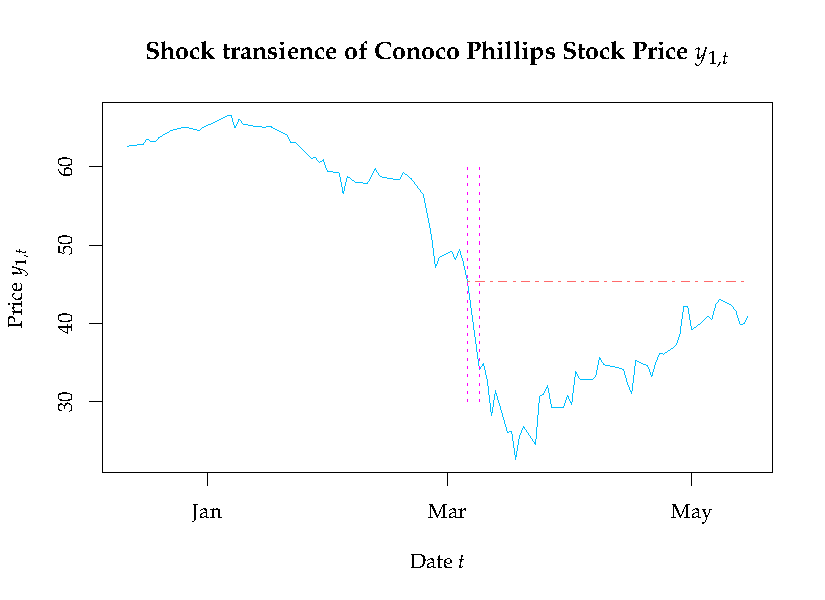
\includegraphics[height = 8cm]{COPtransience.pdf}
		\caption{The shock transience of $\{y_{1,t} \colon 1, \ldots, T_1\}$} \label{copshocktransience}
	\end{center}	
\end{figure}


%\begin{table}[H]
	%\caption{Results for Conoco Philips ($n=5$), $\mbf{W}^* = (0, 0, 0, 0.363, 0.637)$ from scaled covariates}
%\begin{center}
  %\begin{tabular}{cccccccccr}
     %$L$ ($T_i-T^*_i$) & Model & $p_1$  & $|\hat{p}-p_1|$ & Vote & weighted Vote  & weighted  AIC\\
     %\hline 
     %7 & Permanent & 1  & 0 & \textcolor{red}{0}  & \textcolor{red}{0} & $236.21$ \\
     % 7 & Dynamic & 1 & $0$   &  \textcolor{red}{0} & \textcolor{red}{0}  & $324.91$ \\[.2cm]
     %15 & Permanent & 1   & 0 & \textcolor{red}{0} &  \textcolor{red}{0}    & 273.95 \\
     %15 & Dynamic & 1  & 0 & \textcolor{red}{0}  & \textcolor{red}{0}  & $370.83$\\[.2cm]
     %30 & Permanent & 1   & $0$ &  \textcolor{red}{0} & \textcolor{red}{0}  &  346.17 \\
     %30 & Dynamic & 1 & 0 & \textcolor{red}{0} &\textcolor{red}{0}  & 451.16
  %\end{tabular}
%\end{center}	
%\end{table}


\subsection{Testing shock prevalence for Month-on-Month Change in Log Nonfarm Payrolls (Seasonally Adjusted)}

\label{sptuem}

Arguably the most watched macroeconomic indicator for the US economy is the monthly release of the total nonfarm payrolls, which reflects the gains or losses of persons employed.  However, its reputation as a lagging indicator of macroeconomic health constrains its usefulness.  This makes it ripe for forecasting under the method herein.  To this end, we examine the March 2020 lockdown measures as a shock to the US economy and labor market, enlisting previous macroeconomic shocks to the US economy as donors.  The donor pool assembled notably contains no cases of lockdowns or even pandemics or epidemics.  Instead, the common thread running through the time series under study and the donors is the element of a sudden and considerable surprise visited upon the economy from source previously judged to be marginal.

\textcolor{red}{A lot is needed here. We need to say that we are assuming that government lockdowns are temporary or rather that the effect of government lockdowns will be temporary. We need to mention that none of the time series in the donor pool involve lockdowns. We should consider a few time horizons. Something like 2, 3, or 4 months ahead might be interesting (we may need to consider a less complex dynamic model for fitting purposes). I would guess that a shorter window may exhibit disagreement between the donor pool and the series under study or may show different decisions being reported. However, don't we want to match the time series under study with donors based on only pre-shock features, data, variables, etc?  It might be good to think of donor selection as a two-stage matching procedure: first, a donor is judged worthy based on some qualitative or quantitative analysis (the latter of which can be simply the correlation of their covariate vectors at $T^{*}$); second, the matches are aggregated using distanced-based weighting.}


Arguably the most watched macroeconomic indicator for the US economy is the monthly release of the total nonfarm payrolls, which reflects the gains or losses of persons employed. The pandemic-induced recession of 2020 coincided with a one-month drop in US nonfarm payrolls in excess of 20 million people, or $13.57\%$, between March and April 2020.  This decline exceeds all other monthly declines by many orders of magnitude, and hence then distance-based weighting employed in \citep{lin2021minimizing} could not hope to recover the full shock effect.  However, the test developed herein does not rely as heavily upon the assumption of a common shock distribution for donors or the assumption that the donors represent a rich and diverse sampling from that distribution (\textcolor{red}{Think about this}).  Instead, what is needed is that the donor pool serve as an information source about the persistence of a shock effect in the time series under study.  

To that end, we assemble a donor pool of US recessions induced by large shocks in the last three decades: the recessions of 1981-82, 2001-2003, and 2007-2009 (\textcolor{red}{Justification needed for these shocks; the March 2020 lockdown was an unprecedented halting of economic activity}).  We employ a suite of monthly macroeconomic indicators as covariates for the linear model as for arriving at an optimal weighting of the donor pool.  These indicators are all transformed to their month-on-month change in log values, so as to be consistent with the time series under study and to capture the signal inherent in changes, not raw levels, of macroeconomic variables.  These indicators are the US unemployment insurance transfers, real personal income, personal consumption expenditures, industrial production, consumer price index, Federal Reserve funds rate, and the count of black Americans age 20 and over on US nonfarm payrolls.


The variable selection steps are outlined as follows. At first, we have the same set of covariates $\{\mc{X}_1, \ldots, \mc{X}_p\}$ for each donor, where $\mc{X}_1$ corresponds to the name of the covariate. Next, for each donor, we conduct stepwise variable selection based on AIC so that for each donor, we end up with a model with covariates that may differ across  donors, say $\{\mc{X}_j \colon j\in \mc{I}_i\}$ for $i = 2, \ldots, n+1$, where $\mc{I}_j$ is the collection of the indices corresponding to which covariate is selected. Next, we  take the union $\cup_{i=2}^{n+1}\{\mc{X}_j \colon j\in \mc{I}_i\}$ to obtain the final set of covariates that are present in the model of every donor and the time series of interest.

In Table 2, using the synthetic pairwise model selection procedures specified in Corollary \ref{coro2}, because $\sum_{i=2}^4 w_i^* I(a_i^1 > a_i^2)>0.5$,  we conclude that  $\mc{M}$ is preferred. Thus, we turn our interest to that model.  Since $p_{1}$ is far above the rejection threshold, we lack the evidence to reject the null of a transient shock in the time series under study, the month-on-month change in log employment in the span 2019-2022.  The weighted p-value, $\hat p $, misses the ground truth p-value by .146 in absolute value, yet renders the correct decision.




\textbf{Questions to answer and points to hit}
\begin{enumerate}
\item Why did I choose the donors I chose? X 
\item Why did I use the columns I did in OLS? X
\item Why did I use the columns I did in the estimation of the points on the simplex? X
\item Discuss the two models, M1, M2 X
\item Weighted AIC just as in previous example?  X
\item By weighted AIC, M2 is the preferred model Yes
\item We can see that $p_{1}$ is far larger than the rejection threshold, indicating that we lack the evidence to reject the null of a transiet shock
\item The weighted pvalue, $\hat p $, misses the ground truth p-value by .146 in absolute value
\item The method of voting renders the correct decision
\item The method of weighted voting renders the correct decision
\item Ask Jilei to correct y-axis X
\item Ask Jilei whether AIC was used in the same way as first example X
\item Ask Jilei whether covariate set $\textbf{X}$ is same as simplex optimization $\textbf{X}$ 
\item Ask Jilei to drop RPI as a covariate in OLS (but not necessarily for optimization) (needs checking)
\item Ask Jilei to include chart with data stopping at March 2020 to better visualize how payrolls change by month X

\end{enumerate}

\begin{table}[H]
	\caption{Results for Month-on-Month Change in Log Nonfarm Payrolls (Seasonally Adjusted) ($n=3$), $\mbf{W}^* = (0, 0.278, 0.722)$ from scaled covariates} \label{uemtable}
\begin{center}
  \begin{tabular}{cccccccccr}
   $L$  &  Model & $\sum_{i=2}^4 w_i^* I(a_i^1 > a_i^2)$  & $p_1$ &  $|\hat{p}-p_1|$ & Vote (Correct?) & weighted Vote (Correct?)   \\
     \hline 
     \multirow{2}{*}{ $3$} &  $\mc{M}_0$  & \multirow{2}{*}{ 0}& 1  & 0 & 0 (Yes) &0 (Yes)  \\      
      & $\mc{M}$ ($q_1=q_2=1$)  & & 0.070 & $0.179$   & 0 (Yes) &1 (No)   \\[.2cm]
     \multirow{2}{*}{ $6$} &  $\mc{M}_0$  & \multirow{2}{*}{ 0}& 1  & 0 & 0 (Yes) &0 (Yes)  \\      
      & $\mc{M}$ ($q_1=q_2=1$)  & & 0.265 & $0.498$   & 0 (Yes) &0 (Yes)   \\[.2cm]
  \multirow{2}{*}{ $12$} &  $\mc{M}_0$  & \multirow{2}{*}{0.722}& 0  & 1 & 1 (No) &1 (No)  \\      
      & $\mc{M}$ ($q_1=q_2=1$)  & & 0.470 & $0.146$   & 0 (Yes) &0 (Yes)   \\[.2cm]
       \multirow{2}{*}{ $18$} &  $\mc{M}_0$  & \multirow{2}{*}{0}& 0.670  & 0.330 & 0 (Yes) & 0 (Yes)  \\      
      & $\mc{M}$ ($q_1=q_2=1$)  & & 1 & $0$   & 0 (Yes) &0 (Yes)   \\[.2cm]
  \end{tabular}
\end{center}	
\end{table}


\begin{figure}[H]
	\begin{center}
		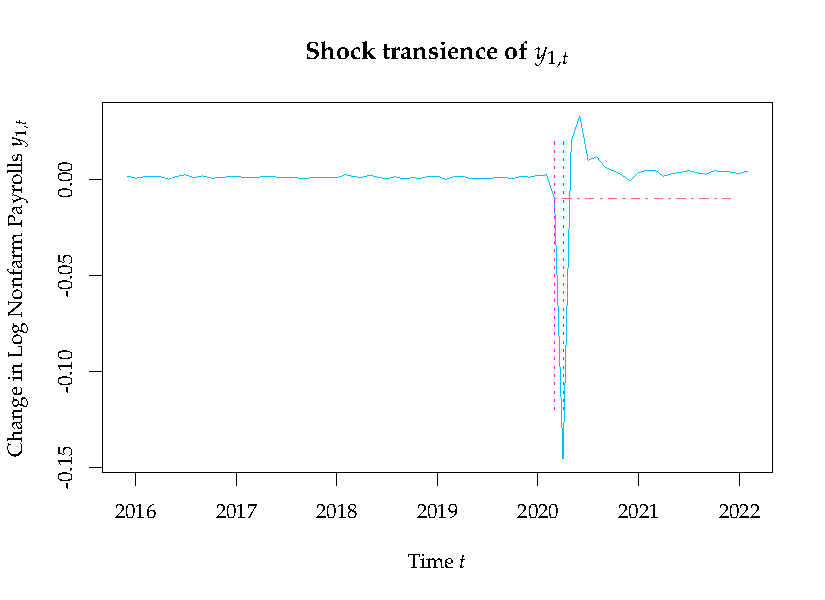
\includegraphics[height = 8cm]{UEMtransience.pdf}
		\caption{The shock transience of $\{y_{1,t} \colon 1, \ldots, T_1\}$} \label{uemshocktransience}
	\end{center}	
\end{figure}



\subsection{Simulations}
\label{simulation}




\section{Discussion}

Talk about post-shock forecasting as parameterizing exogeniety and using hindsight in the donor pool to explicitly estimate exogeneity apriori. This framing has its limits, we are not able to perform post-shock forecasts when we are temporarily removed from the known shock time. For example, in the Conoco Philips analysis it is hard to imagine a successful post-shock forecast being made in the days prior to the weekend preceding Monday, March 9th 2020 as the OPEC-Russia oil supply increases and Covid-19 fears had not yet taken shape.

The post-shock forecasting methodology presented here and in \cite{lin2021minimizing} is heavily dependent on the construction of a suitable donor pool which will exhibit a degree of subjectivity. This is a limitation of our approach, but we argue that this limitation is not a deal breaker.  



\section{Mathematical Appendix}


Proof of Proposition~\ref{votprop}:

\begin{proof}
Notice that as $\P(p_i \leq \alpha)=\kappa$ for $i = 1, \ldots, n+1$ and $I(p_i \leq  \alpha) $ is a Bernoulli random variable, $I(p_i \leq  \alpha)$ is identically distributed for  $i = 1, \ldots, n+1$. Since $p_i$ is pairwise independent and $p_i$ are identically distributed for $i = 2, \ldots, n+1$, by Weak Law of Large Numbers, 
\begin{align*}
  \frac{1}{n}\sum_{i=2}^{n+1}I(p_i \leq  \alpha)  
   \stackrel{p}{\rightarrow}  \P(p_i \leq \alpha) = \P(p_1 \leq \alpha),
\end{align*}
Define
\begin{align*}
  f \colon [0,1] \mapsto \{0,1\} 
  \text{ with }
  f(x) = I(x \geq 0.5).
\end{align*}
Let $C(f)$ denote the continuity set of $f$. Suppose that $\P(p_1 \leq  \alpha) \neq 0.5$. In this case, notice that 
\begin{align*}
  \P(\P(p_1 \leq  \alpha) \in C(f)) =1.
\end{align*}
By Slutsky's Theorem, we have
\begin{align*}
  I\left\{\frac{1}{n}\sum_{i=2}^{n+1}I(p_i \leq  \alpha) \geq 0.5\right\}
  \stackrel{p}{\rightarrow} 
  I\{ \P(p_1 \leq  \alpha) \geq 0.5\}.
\end{align*}
It follows that
\begin{align*}
   I\left\{\frac{1}{n}\sum_{i=2}^{n+1}I(p_i \leq  \alpha) \geq 0.5\right\}- I( p_1 \leq  \alpha) 
  \stackrel{p}{\rightarrow} 
  I\{ \P(p_1 \leq  \alpha) \geq 0.5\} - I( p_1 \leq  \alpha) 
\end{align*}
Since the function $g(x)= |x|$ is continuous in $x$,  by continuous mapping theorem, 
\begin{align*}
  \bigg|  I\left\{\frac{1}{n}\sum_{i=2}^{n+1}I(p_i \leq  \alpha) \geq 0.5\right\}
  - I( p_1 \leq  \alpha) \bigg| \stackrel{p}{\rightarrow}   |I\{ \P(p_1 \leq  \alpha) \geq 0.5\}
  - I( p_1 \leq  \alpha) |
\end{align*}
Moreover, note that
\begin{align*}
\E \left\{ |I\{ \P(p_1 \leq  \alpha) \geq 0.5\}
  - I( p_1 \leq  \alpha) |\right\}
  & = \begin{cases}
    1- \P(p_1 \leq \alpha) & \text{ if } \P(p_1 \leq \alpha) > 0.5 \\
    \P(p_1 \leq \alpha) & \text{ if } \P(p_1 \leq \alpha) < 0.5 
  \end{cases} \\
  & \leq  0.5.
\end{align*}
Due to the fact that
\begin{align*}
 \left|I\left\{\frac{1}{n}\sum_{i=2}^{n+1}I(p_i \leq  \alpha) \geq 0.5\right\}
  - I( p_1 \leq  \alpha) \right| \leq 1
\end{align*}
is bounded by 1, by Dominated Convergence Theorem for the version of convergence in measure,
\begin{align*}
 \left|I\left\{\frac{1}{n}\sum_{i=2}^{n+1}I(p_i \leq  \alpha) \geq 0.5\right\}
  - I( p_1 \leq  \alpha) \right|
  \stackrel{\mathcal{L}_1}{\rightarrow}  |I\{ \P(p_1 \leq  \alpha) \geq 0.5\}
  - I( p_1 \leq  \alpha) |.
\end{align*}
That would imply that 
\begin{align*}
  \E \bigg\{\left|I\left\{\frac{1}{n}\sum_{i=2}^{n+1}I(p_i \leq  \alpha) \geq 0.5\right\}
  - I( p_1 \leq  \alpha) \right|\bigg\}
  \to  \begin{cases}
    1- \P(p_1 \leq \alpha) & \text{ if } \P(p_1 \leq \alpha) > 0.5 \\
    \P(p_1 \leq \alpha) & \text{ if } \P(p_1 \leq \alpha) < 0.5 
  \end{cases}
\end{align*}
That is, the expected misclassification rate of voting converges to 
\begin{align*}
  \begin{cases}
    1- \P(p_1 \leq \alpha) & \text{ if } \P(p_1 \leq \alpha) > 0.5 \\
    \P(p_1 \leq \alpha) & \text{ if } \P(p_1 \leq \alpha) < 0.5 
  \end{cases}
\end{align*}
\end{proof}


We now provide a proof for Proposition~\ref{votprop2}. This proof requires a lemma from probability theory whose proof we include for completeness.

\begin{lem}
  \label{gwlln}  For each $n\in \naturals$, let $c_{n1}, \ldots, c_{nn}$ be real numbers bounded by some $K > 0$, and let $X_{n1}, \ldots, X_{nn}$ be pairwise independent random variables defined on a probability space $(\Omega_n, \mc{F}_n, \P_n)$, and let $\E_n$ and $\var_n$ denote the corresponding expectation and variance. If $(b_n)$ is a sequence of positive numbers such that $b_n \uparrow \infty$ such that
    \begin{align*}
      \sum_{i=1}^n \P_n (|X_{ni}| > b_n) \to 0
      \quad \text{ and } 
      \quad \frac{1}{(b_n)^2} \sum_{i=1}^n \E_n[X_{ni}^2; |X_{ni}|\leq b_n] \to 0,
    \end{align*}
    then
    \begin{align*}
      \frac{1}{b_n} \sum_{i=1}^n c_{ni} (X_{ni} - \E_n[X_{ni}; X_{ni} \leq b_n]) \cp 0.
    \end{align*}
\end{lem}

\begin{proof}
  For each $n\in \naturals$ set
    \begin{align*}
      S_n = \sum_{i=1}^n c_{ni} X_{ni}, \quad T_n = \sum_{i=1}^n c_{ni} Y_{ni},
      \quad Y_{ni} = X_{ni} I(|X_{ni}|\leq b_n), \quad i = 1, \ldots, n.
    \end{align*}
   The goal is to show that  $(S_n- \E_n[T_n])/b_n \cp 0$. For this, it suffices to show that (1) $(T_n - S_n)/b_n \cp 0$ and (2) $(T_n - \E_n[T_n])/b_n \cp 0$ because
    \begin{align*}
      (T_n - \E_n[T_n])/b_n -(T_n - S_n)/b_n = (S_n- \E_n[T_n])/b_n .
    \end{align*}
     We first prove (1). Notice that for every $\varepsilon > 0$ and $n\in \naturals$,
    \begin{align*}
      \{|S_n- T_n| > \varepsilon\}\subseteq \bigcup_{i=1}^n \{X_{ni}\neq Y_{ni}\}
      = \bigcup_{i=1}^n \{|X_{ni}|>b_n\},
    \end{align*}
    and, as a result, by Boole's inequality we have
    \begin{align*}
      \P_n (|S_n - T_n|>\varepsilon) \leq \sum_{i=1}^n \P_n(|X_{ni}|>b_n) \to 0,
    \end{align*}
    which proves (1). Next, we prove (2). Since $\mc{L}^2$ implies convergence in probability, it suffices to show that $(T_n-\E[T_n])/b_n \clt 0$, i.e., $\var[T_n]/(b_n)^2 \to 0$. Since $X_{n1}, \ldots, X_{nn}$ are pairwise independent, so are $Y_{n1}, \ldots, Y_{nn}$, and consequently
    \begin{align*}
      \Var_n[T_n]=\sum_{i=1}^n \Var_n[Y_{ni}] \leq \sum_{i=1}^n \E_n[(c_{ni}X_{ni})^2; |X_{ni}|\leq b_n] \leq K^2\sum_{i=1}^n \E_n[(X_{ni})^2; |X_{ni}|\leq b_n].
    \end{align*}
    As a result,
    \begin{align*}
    0\leq   \frac{\Var_n[T_n]}{b_n^2}\leq K^2 \cdot  \frac{1}{b_n^2}\sum_{i=1}^n \E_n[(X_{ni})^2; |X_{ni}|\leq b_n] \to 0,
    \end{align*}
    which proves the result by sandwich theorem.
\end{proof}

We now have enough to prove Proposition \ref{votprop2}:

\begin{proof}
  The proof is rather similar to Proposition \ref{votprop}. It suffices to show that
  \begin{align*}
   \sum_{i\in \mc{I}_n} w_i I(p_i \leq  \alpha) \cp \kappa_1 =  \P(p_1 \leq \alpha).
  \end{align*}
  and the remaining proof is the same as that of Proposition \ref{votprop} in terms of applying Dominated Convergence Theorem in the version of  convergence in probability. As $p_i$ are pairwise independent for $i\in \mc{I}_n$, $I(p_i\leq \alpha)$ are pairwise independent for $i \in \mc{I}_n$. The idea is to prove the required condition of Lemma \ref{gwlln} holds. As  $\mc{I}_n$  is non-empty, $|\mc{I}_n| \to \infty$, $b_n > 1$, and  $b_n \to \infty$ as $n \to \infty$, 
  \begin{align*}
    & \sum_{i\in \mc{I}_n} \P\big( I(p_i \leq  \alpha) > b_n\big) \to 0\\
   & \frac{1}{b_n^2} \sum_{i\in \mc{I}_n} \E\big[ I(p_i \leq  \alpha) \,|\, I(p_i \leq  \alpha) \leq b_n\big]
     =  \frac{1}{b_n^2} \sum_{i\in \mc{I}_n} \P\big(p_i \leq\alpha \big)
     = \frac{1}{b_n^2} \sum_{i\in \mc{I}_n} w_i \kappa_i  \to 0
  \end{align*}
  because $ \sum_{i\in \mc{I}_n} w_i \kappa_i = O(1)$ by the assumption $\sum_{i\in \mc{I}_n} w_i \kappa_i \to \kappa_{1}$. Let $c_{ni} = w_i b_n$ for $i \in \mc{I}_n$. Since $w_i b_n\leq K$ for some $K > 0$ and $b_n$, we have 
  \begin{align*}
    & \frac{1}{b_n} \sum_{i\in \mc{I}_n}  c_{ni} \big(  I(p_i \leq  \alpha) - \P( I(p_i \leq  \alpha) \, |\,  I(p_i \leq  \alpha)  \leq b_n )  \big) \\
  = \quad     &\frac{1}{b_n} \sum_{i\in \mc{I}_n}  c_{ni} \big(  I(p_i \leq  \alpha) - \P( I(p_i \leq  \alpha) \big)  \cp 0
  \end{align*}
  which follows from Lemma \ref{gwlln}. The above is equivalent to
  \begin{align*}
   \sum_{i\in \mc{I}_n}  w_i I(p_i \leq  \alpha) - \sum_{i\in \mc{I}_n} w_i  \kappa_i  \cp 0
  \end{align*}
  As $\sum_{i\in \mc{I}_n} w_i  \kappa_i\to \kappa_1$ as $n \to \infty$, by Slutsky's Theorem,
  \begin{align*}
     \sum_{i\in \mc{I}_n}  w_i I(p_i \leq  \alpha)  \cp \kappa_1,
  \end{align*}
  which finishes the proof.
\end{proof}




\bibliographystyle{plainnat}
\bibliography{synthetic-prediction-notes}
%\bibliography{../synthetic-prediction-notes}

	
\end{document}


